% Provenance (never printed): see sources/outline_sources.md (Year 1: grain size and sorting;
% bedforms and sedimentary structures; fluvial, deltaic, shoreline and deep-sea deposits).
% Exercise and problem values in the Book 3 scratch calculator calc/ch21.py; figure data
% from figdata/bachelor-1/grain_size.py. Meander and delta are Book 1's (g5), sediment and
% sedimentary layer Book 1's (g7), beach Book 1's (g9); the loads, settling, the threshold
% of motion and the Hjulstrom diagram are ch. 20's; the vector mean is ch. 6's. Facies
% models and Walther's law belong to the Year 3 volume (prose pointer only). Pelagic
% sediments are ch. 22's.
\chapter{Sedimentos clásticos y sus ambientes}\label{ch:b1:clastic-sediments}

Recoja un puñado de arena de una playa y déjelo correr entre los dedos: los granos tienen casi todos el mismo tamaño, redondeados y limpios, y fluyen como el agua.
A unos cientos de kilómetros tierra adentro, al pie de una colina dejada por un antiguo glaciar, el terreno es una mezcla rígida de bloques, cantos, arena y lodo,
sin orden. Los dos depósitos están hechos del mismo tipo de detritos, rotos de los mismos tipos de roca; lo que los separa es cómo viajaron los granos y dónde
llegaron a reposar. Una ola que sube y baja por una playa miles de veces al día clasifica los granos por tamaño, se lleva los finos y redondea el resto; el hielo
arrastra todo lo que recoge y lo deja caer en bloque cuando se funde. Este capítulo aprende a leer esas historias en los propios granos, en las estructuras que
construyen en los lechos de ríos y mares, y en el orden en que se apilan los depósitos.

\begin{recall}
Un sedimento es un material suelto depositado por el agua, el viento o el hielo, y con el tiempo los sedimentos se apilan en capas que se endurecen en roca
sedimentaria (libro 1, años 6 y 7). Un río que oscila de un lado a otro de su llanura de inundación forma meandros; donde entra en el mar o en un lago y suelta su
carga, construye un delta; las olas amontonan arena en playas y la desplazan a lo largo de la costa por la deriva litoral (libro 1, años 5 y 9). Un río transporta su
carga como \omterm{def:b1:erosion-transport:load}{carga de fondo}, \omterm{def:b1:erosion-transport:load}{carga en suspensión} y \omterm{def:b1:erosion-transport:load}{carga disuelta}; un grano se hunde a su \omterm{def:b1:erosion-transport:settling}{velocidad de sedimentación}; empieza a moverse cuando el \omterm{def:b1:erosion-transport:bed-shear}{esfuerzo de cizalla en
el fondo} supera su \omterm{def:b1:erosion-transport:threshold}{umbral de movimiento}, y el \omterm{def:b1:erosion-transport:hjulstrom}{diagrama de Hjulström} muestra las velocidades medias de erosión, transporte y sedimentación frente al tamaño del grano
(\cref{ch:b1:erosion-transport}). El vector medio de un conjunto de direcciones es la dirección de la suma de sus vectores unitarios
(\cref{def:b1:field-lab-methods-1:mean-orientation}).
\end{recall}

\section{Tamaño de grano y clasificación}\label{sec:b1:clastic-sediments:grain-size}

El tamaño de los granos es lo primero que anota un geólogo en un sedimento clástico, formado por fragmentos de rocas más antiguas, porque mide la energía de la
corriente que los depositó. Los tamaños de grano en la naturaleza abarcan más de siete órdenes de magnitud, desde bloques de metros de diámetro hasta partículas de
arcilla de una milésima de milímetro de anchura, y se miden en una escala de cocientes.

\begin{definition}[Escala de tamaños de grano, escala phi]\label{def:b1:clastic-sediments:grain-size}
La \emph{escala de tamaños de grano}\index{escala de tamaños de grano} de la sedimentología divide los diámetros de los granos en clases cuyos límites se duplican de
una clase a la siguiente, a partir de \qty{1}{mm}; cada clase tiene un nombre (arena, limo\ldots). La \emph{escala phi}\index{escala phi} expresa un diámetro $d$ mediante
\[
  \varphi = -\log_2 \frac{d}{\qty{1}{mm}},
\]
así que $d = 2^{-\varphi}$~mm: \qty{1}{mm} es $\varphi = 0$, \qty{2}{mm} es
$\varphi = -1$, \qty{0.25}{mm} es $\varphi = 2$, y los granos más finos tienen valores
mayores de $\varphi$.
\end{definition}
% ledger: folk:udden-krumbein, folk:wentworth-classes, usgs:wentworth-phi

En la \omterm{def:b1:clastic-sediments:grain-size}{escala phi} cada clase de la \omterm{def:b1:clastic-sediments:grain-size}{escala de tamaños de grano} tiene una unidad de anchura: una clase que va de $d$ a $2d$ va de $\varphi$ a $\varphi - 1$. Las clases
principales, con los nombres de uso común, figuran en \cref{tab:b1:clastic-sediments:classes}.

\begin{table}[htbp]
\centering\small
\begin{tabular}{@{}lll@{}}
\hline
clase & diámetro (\si{mm}) & $\varphi$ \\
\hline
bloque & por encima de 256 & por debajo de $-8$ \\
canto rodado & de 64 a 256 & de $-6$ a $-8$ \\
guijarro & de 4 a 64 & de $-2$ a $-6$ \\
gránulo & de 2 a 4 & de $-1$ a $-2$ \\
arena (muy gruesa, gruesa, media, fina, muy fina) & de $1/16$ a 2 & de 4 a $-1$ \\
limo (grueso, medio, fino, muy fino) & de $1/256$ a $1/16$ & de 8 a 4 \\
arcilla & por debajo de $1/256$ (\qty{3.9}{\micro m}) & por encima de 8 \\
\hline
\end{tabular}
\caption{Las clases granulométricas. Las cinco clases de arena tienen cada una una unidad phi de anchura, desde muy gruesa (de 1 a \qty{2}{mm}) hasta muy
fina ($1/16$ a $1/8$~mm), y lo mismo las cuatro clases de limo. Algunos autores ponen el límite inferior del limo en 9 en lugar de $8\,\varphi$. La grava es el
nombre general de los granos más gruesos que \qty{2}{mm}, y el fango, la mezcla de limo y arcilla.}
\label{tab:b1:clastic-sediments:classes}
\end{table}
% ledger: folk:wentworth-classes, usgs:wentworth-phi

La palabra \emph{arcilla} tiene dos significados en este libro: aquí es una clase de tamaño, en \cref{ch:b1:weathering-clays} una familia de \omterm{def:b1:rock-forming-minerals:mineral}{minerales}. La
mayoría de las partículas del tamaño de la arcilla son \omterm{def:b1:rock-forming-minerals:mineral}{minerales} de arcilla, y la mayoría de los \omterm{def:b1:rock-forming-minerals:mineral}{minerales} de arcilla son del tamaño de la arcilla, pero los
dos conjuntos no coinciden: el cuarzo molido muy fino tiene tamaño de arcilla, y un libro de \omterm{def:b1:weathering-clays:clay-mineral}{caolinita} puede tener el tamaño del limo.

\emph{Medición de los tamaños.} La grava se mide grano a grano con calibres. La arena se tamiza: se agita una pila de tamices con mallas en cada unidad
phi entera o media, y se pesa lo retenido por cada tamiz. El limo y la arcilla, más finos que $4\,\varphi$, se miden por sedimentación: el sedimento se agita en agua,
y como cada grano se hunde a una velocidad fijada por su tamaño (ley de Stokes, \cref{prop:b1:erosion-transport:stokes}), la masa que sigue en suspensión a una
profundidad y un tiempo dados indica qué fracción de la muestra es más fina que un diámetro dado. Los instrumentos láser que miden la dispersión de la luz por los
granos son también comunes ya. El resultado es una lista del peso por ciento en cada clase.

\begin{definition}[Tamaño medio de grano, clasificación]\label{def:b1:clastic-sediments:sorting}
Sea la distribución de los tamaños de grano de un sedimento, en unidades phi, dada por el peso en cada clase. Su \emph{tamaño medio de grano}\index{tamaño medio de grano}
es la media de esa distribución, y su \emph{clasificación}\index{clasificación} es la dispersión de la distribución, medida por su desviación típica en unidades phi: un
sedimento está bien clasificado cuando sus granos son casi todos de un mismo tamaño, y mal clasificado cuando cubren muchas clases. Ambos se calculan, o bien a
partir de los porcentajes en las clases, por el método de los momentos, o bien a partir de la curva acumulada, con las medidas gráficas de Folk:
\[
  M_z = \frac{\varphi_{16} + \varphi_{50} + \varphi_{84}}{3}, \qquad
  \sigma_I = \frac{\varphi_{84} - \varphi_{16}}{4} + \frac{\varphi_{95} - \varphi_{5}}{6.6},
\]
donde $\varphi_p$ es el tamaño en unidades phi por debajo del cual el $p$ por ciento de la muestra es más grueso.
\end{definition}
% ledger: folk:graphic-measures

\begin{method}[Media y clasificación a partir de un análisis por tamizado]\label{met:b1:clastic-sediments:graphic}
\begin{enumerate}
  \item Enumérense los porcentajes en peso $w_i$ en cada clase, de la más gruesa a la más fina, y compruébese que la suma es \qty{100}{\percent} (o divídase entre ella).
  \item \emph{Método de los momentos.} Con $x_i$ el punto medio de la clase $i$ en unidades phi, calcúlese la media $m = \sum w_i x_i / 100$ y la desviación típica
        $s = \sqrt{\sum w_i (x_i - m)^2 / 100}$.
  \item \emph{Medidas gráficas.} Acumúlense los porcentajes para obtener el peso por ciento más grueso que cada límite de clase, y represéntese frente a $\varphi$:
        esta es la curva acumulada.
  \item Léanse en ella, por interpolación lineal entre los límites de clase, los tamaños $\varphi_5$, $\varphi_{16}$, $\varphi_{50}$, $\varphi_{84}$ y
        $\varphi_{95}$.
  \item Calcúlense $M_z$ y $\sigma_I$ (\cref{def:b1:clastic-sediments:sorting}), conviértase $M_z$ a milímetros mediante $d = 2^{-M_z}$, y nómbrese la \omterm{def:b1:clastic-sediments:sorting}{clasificación}
        según la escala de abajo.
\end{enumerate}
\end{method}

Los dos métodos dan respuestas casi iguales, y la razón es la siguiente propiedad.

\begin{proposition}[Medidas gráficas de una distribución normal]\label{prop:b1:clastic-sediments:normal}
Si los tamaños de un sedimento, en unidades phi, se distribuyen normalmente con media
$\mu$ y desviación típica $\sigma$, entonces $M_z = \mu$ y $\sigma_I = 0.996\,\sigma$.
\end{proposition}

\begin{proof}
Para una distribución normal, la fracción de valores por debajo de $\mu + z\sigma$ depende
solo de $z$; la fracción por debajo de $\mu + 0.9945\,\sigma$ es el \qty{84}{\percent}
y por debajo de $\mu + 1.6449\,\sigma$ es el \qty{95}{\percent} (valores de la distribución normal, admitidos). Por simetría, $\varphi_{50} = \mu$, $\varphi_{16} = \mu -
0.9945\,\sigma$, $\varphi_{84} = \mu + 0.9945\,\sigma$, $\varphi_5 = \mu -
1.6449\,\sigma$ y $\varphi_{95} = \mu + 1.6449\,\sigma$ (los percentiles cuentan
la parte más gruesa, es decir, el $\varphi$ menor, pero la distribución es
simétrica). Entonces $M_z = (3\mu)/3 = \mu$ y
\[
  \sigma_I = \frac{2 \times 0.9945\,\sigma}{4} + \frac{2 \times 1.6449\,\sigma}{6.6}
  = (0.4972 + 0.4985)\,\sigma = 0.996\,\sigma. \qedhere
\]
\end{proof}

La constante 6.6 de la fórmula de Folk se eligió para esto: el intervalo del 5.º al 95.º percentil abarca $3.29$ desviaciones típicas de una distribución
normal, y la fórmula promedia las estimaciones de $\sigma$ de los dos intervalos, $(\varphi_{84}-\varphi_{16})/2$ y $(\varphi_{95}-\varphi_5)/3.3$.
Usar las colas además de las dos terceras partes centrales de la curva hace que $\sigma_I$ sea sensible a las mezclas gruesas y finas que más dicen sobre cómo
se depositó un sedimento.

\begin{omfigure}
\begin{tikzpicture}[font=\small]
% grain-size histograms and cumulative curves of two invented samples (figdata/bachelor-1/grain_size.py)
\begin{axis}[name=a, width=7.3cm, height=6cm, xmin=-5.5, xmax=10.5, ymin=0, ymax=90,
    xlabel={tamaño de grano $\varphi$}, ylabel={porcentaje en peso de la clase},
    title={\footnotesize (a) histogramas}, xtick={-4,-2,...,10}, ytick={0,20,...,80},
    legend style={at={(0.03,0.97)}, anchor=north west, font=\scriptsize}, legend cell align=left]
  \addplot[ybar interval, fill=omDef!35, draw=omDef, area legend] table[x=phi, y=wt] {figdata/out/bachelor-1-grain_size-step-beach.dat} \closedcycle;
  \addplot[const plot, fill=omThm!20, draw=omThm, fill opacity=0.6, area legend] table[x=phi, y=wt] {figdata/out/bachelor-1-grain_size-step-till.dat} \closedcycle;
  \legend{arena de playa (clases de medio phi), till (clases de phi entero)}
\end{axis}
\begin{axis}[at={(a.east)}, anchor=west, xshift=1.6cm, width=7.3cm, height=6cm, xmin=-5.5, xmax=10.5, ymin=0, ymax=100,
    xlabel={tamaño de grano $\varphi$}, ylabel={porcentaje en peso más grueso},
    title={\footnotesize (b) curvas acumuladas}, xtick={-4,-2,...,10}, ytick={0,16,50,84,100},
    grid=major, grid style={black!10}]
  \addplot[omDef, very thick, mark=*, mark size=1.2pt] table[x=phi, y=cum] {figdata/out/bachelor-1-grain_size-cum-beach.dat};
  \addplot[omThm, very thick, mark=*, mark size=1.2pt] table[x=phi, y=cum] {figdata/out/bachelor-1-grain_size-cum-till.dat};
  \node[font=\footnotesize, omDef, anchor=west] at (axis cs:2.9,40) {arena de playa};
  \node[font=\footnotesize, omThm, anchor=west] at (axis cs:5.4,72) {till};
\end{axis}
\end{tikzpicture}

{\small Las distribuciones de tamaño de dos sedimentos, a partir de análisis por tamizado y por sedimentación (datos inventados). (a)~Porcentaje en peso en
cada clase: la arena de playa cae casi por completo en tres clases de medio phi de arena media y fina; el till se extiende sobre quince clases phi, desde guijarros
hasta arcilla. (b)~Las curvas acumuladas, porcentaje en peso más grueso que cada tamaño: cuanto más empinada la curva, mejor la \omterm{def:b1:clastic-sediments:sorting}{clasificación}. Las medidas gráficas
leídas al 5, 16, 50, 84 y 95 por ciento dan, para la arena, $M_z = 2.25\,\varphi$ (\qty{0.21}{mm}) y $\sigma_I =
0.36\,\varphi$, y para el till $M_z = 1.83\,\varphi$ y $\sigma_I = 3.84\,\varphi$.}
\label{fig:b1:clastic-sediments:grain-size}
\end{omfigure}
% ledger: folk:graphic-measures

\emph{Palabras para la \omterm{def:b1:clastic-sediments:sorting}{clasificación}.} A partir de muchos sedimentos medidos, Folk propuso una escala verbal para $\sigma_I$: por debajo de \num{0.35}, muy bien clasificado;
de \num{0.35} a \num{0.50}, bien clasificado; de \num{0.50} a \num{0.71}, moderadamente bien clasificado; de \num{0.71} a \num{1.0}, moderadamente clasificado; de \num{1.0}
a \num{2.0}, mal clasificado; de \num{2.0} a \num{4.0}, muy mal clasificado, y por encima de \num{4.0}, extremadamente mal clasificado. La mejor \omterm{def:b1:clastic-sediments:sorting}{clasificación} que alcanzan
los sedimentos naturales es de unos \num{0.20} a \num{0.25}, y las arenas de \omterm{def:b1:clastic-sediments:bedform}{dunas} y playas que él midió estaban entre \num{0.25} y \num{0.35}; los sedimentos de ríos
iban de \num{0.40} a \num{2.5}, los limos y arcillas de llanuras de inundación y plataformas de unos \num{2.0} a \num{3.5}, y los más mal clasificados de todos eran los
tills glaciares y los flujos de lodo. La arena de playa de la figura, con \num{0.36}, está bien clasificada, en el límite de muy bien clasificada; el till, con
\num{3.84}, muy mal clasificado. En el till el método de los momentos da una media de $1.89\,\varphi$ y una desviación típica de $3.64\,\varphi$, cerca de los valores
gráficos; las diferencias proceden de las colas y de la asimetría de la distribución.
% ledger: folk:sorting-classes, folk:natural-sorting

La \omterm{def:b1:clastic-sediments:sorting}{clasificación} es un registro del transporte. Una corriente clasifica su carga porque los granos que puede mover, y mantener en suspensión, dependen de su tamaño
(\cref{sec:b1:erosion-transport:threshold}): las olas en una playa y el viento sobre una \omterm{def:b1:clastic-sediments:bedform}{duna} trabajan los mismos granos una y otra vez, quitando los más finos y dejando
los demasiado pesados para moverse, y sus depósitos son los mejor clasificados de todos. El hielo, los flujos de escombros y el vertido súbito de una crecida no clasifican nada.

\emph{Forma y redondez.} La redondez de un grano describe la agudeza de sus esquinas, con independencia de su forma global: Wadell la definió como el radio medio de
curvatura de las esquinas dividido por el radio del mayor círculo inscrito en el contorno del grano, de 1 para una esfera hasta casi 0 para una astilla. Medirla es
tedioso, y los granos se comparan en cambio con cuadros de fotografías; en la escala de Wadell la mayoría de los granos de arena tienen redondeces de \num{0.3} a \num{0.4},
y en la escala logarítmica de Folk, de 0 (muy angular) a 6 (muy redondeado), unos \num{2.5}, subangular. El redondeo es lento en la arena: el cuarzo transportado por el viento
se redondea mucho más deprisa que el cuarzo transportado por el agua, que amortigua los impactos, y la arena de playa más deprisa que la de río, mientras que los granos de arena
apenas se redondean en los ríos. Los cantos se redondean deprisa en los ríos, los blandos primero: en el río Colorado, los cantos de caliza alcanzan su redondez final en unas
pocas millas, mientras que los cantos de cuarzo necesitan unas \num{150} millas para alcanzarla.
% ledger: folk:roundness, folk:rounding

\begin{definition}[Madurez textural, madurez composicional]\label{def:b1:clastic-sediments:maturity}
La \emph{madurez textural}\index{madurez textural} de una arena o de una arenisca mide hasta qué punto la \omterm{def:b1:clastic-sediments:sorting}{clasificación}, la abrasión y el cribado de la corriente han
actuado sobre ella, en cuatro etapas: \emph{inmadura}, con más de \qty{5}{\percent} de matriz arcillosa; \emph{submadura}, con menos arcilla pero granos mal clasificados
($\sigma > 0.5\,\varphi$); \emph{madura}, con poca o ninguna arcilla y bien clasificada ($\sigma < 0.5\,\varphi$) pero con granos angulosos;
\emph{supermadura}, sin arcilla y con granos a la vez bien clasificados y bien redondeados. Su \emph{madurez composicional}\index{madurez composicional} mide hasta qué punto
se han eliminado los \omterm{def:b1:rock-forming-minerals:mineral}{minerales} inestables y los fragmentos de roca, dejando el cuarzo: es alta en una arenisca de cuarzo casi puro y baja en una rica en \omterm{def:b1:rock-forming-minerals:groups}{feldespato}, \omterm{def:b1:rock-forming-minerals:groups}{mica} o
fragmentos de roca.
\end{definition}
% ledger: folk:maturity, folk:mineral-maturity

La \omterm{def:b1:clastic-sediments:maturity}{madurez textural} se lee en el depósito tal como se formó: los \omterm{def:b1:rock-forming-minerals:mineral}{minerales} de arcilla que cristalizaron después en los poros, y los cementos que unen los granos
(\cref{ch:b1:diagenesis-basins}), no cuentan. Refleja la energía del lugar de depósito: los sedimentos inmaduros se acumulan en llanuras de inundación, abanicos aluviales
y lagunas, donde las corrientes son débiles o el depósito demasiado rápido para que los granos se trabajen, y los supermaduros en playas y \omterm{def:b1:clastic-sediments:bedform}{dunas} del desierto, donde la energía
se gasta en los granos sin fin. La \omterm{def:b1:clastic-sediments:maturity}{madurez composicional} sigue de la abrasión y de la meteorización a la vez. El \omterm{def:b1:rock-forming-minerals:groups}{feldespato}, más blando que el cuarzo y con un buen \omterm{def:b1:faults-folds-fabrics:foliation}{clivaje},
se desgasta más deprisa; una arcosa de cuarzo y \omterm{def:b1:rock-forming-minerals:groups}{feldespato} angulosos del mismo tamaño puede, por la abrasión sola, acabar en una arenisca supermadura en la que la arena es casi
toda cuarzo y el \omterm{def:b1:rock-forming-minerals:groups}{feldespato} sobrevive solo como limo. La meteorización, en el área de origen y durante un almacenamiento largo en el camino, hace lo mismo al convertir los
\omterm{def:b1:rock-forming-minerals:groups}{feldespatos} en arcilla (\cref{sec:b1:weathering-clays:hydrolysis}). Las areniscas depositadas en épocas de agitación de la \omterm{def:b1:layered-earth:layers}{corteza}, erosionadas deprisa de montañas en
ascenso, tienden a ser inmaduras en ambos sentidos; las de épocas tranquilas, retrabajadas durante mucho tiempo, tienden a ser areniscas de cuarzo supermaduras; pero las
excepciones son numerosas, y cualquier composición puede darse en cualquier etapa de \omterm{def:b1:clastic-sediments:maturity}{madurez textural}.
% ledger: folk:maturity, folk:mineral-maturity

\section{Formas de fondo y estructuras sedimentarias}\label{sec:b1:clastic-sediments:bedforms}

Cuando una corriente mueve arena sobre un fondo, el fondo rara vez se queda plano: se organiza en ondas de arena que viajan con el flujo. Estas formas, y la estratificación
que dejan dentro del depósito, son el registro más directo de las corrientes del pasado.

\begin{definition}[Forma de fondo, rizo, duna]\label{def:b1:clastic-sediments:bedform}
Una \emph{forma de fondo}\index{forma de fondo} es un relieve regular moldeado por una corriente sobre un fondo de granos sueltos, repetido a lo largo del flujo. Un
\emph{rizo}\index{rizo} es una forma de fondo pequeña, de unos pocos centímetros de altura y de 10 a \qty{20}{cm} de cresta a cresta, con un lado aguas arriba (de ataque)
suave y un lado aguas abajo (de sotavento) empinado; una \emph{duna}\index{duna} tiene una forma parecida pero es al menos diez veces mayor, de decímetros a metros de altura bajo el agua.
\end{definition}
% ledger: southard:ripples-dunes

El lado de ataque de un \omterm{def:b1:clastic-sediments:bedform}{rizo} tiene una pendiente de menos de unos \ang{10}; su lado de sotavento, la cara de deslizamiento, se sitúa cerca del ángulo de reposo de la arena en el agua,
unos \ang{30}. La arena se erosiona del lado de ataque, se lleva por encima de la cresta, y avalancha hacia abajo o cae sobre la cara de deslizamiento, así que todo el \omterm{def:b1:clastic-sediments:bedform}{rizo} se mueve aguas
abajo, mucho más despacio que el agua, tomando granos de su parte trasera y añadiéndolos a su frente. El viento forma \omterm{def:b1:clastic-sediments:bedform}{rizos} y \omterm{def:b1:clastic-sediments:bedform}{dunas} del mismo tipo en tierra, siendo las \omterm{def:b1:clastic-sediments:bedform}{dunas} de los
desiertos mucho mayores que las de los ríos.
% ledger: southard:ripples-dunes, southard:climb

\begin{proposition}[Migración de formas de fondo y carga de fondo]\label{prop:b1:clastic-sediments:migration}
Un tren de \omterm{def:b1:clastic-sediments:bedform}{formas de fondo} de perfil triangular, de altura $H$, que se mueve aguas abajo a la velocidad $c$ sin cambiar de forma, por erosión de los lados de ataque y
depósito en los de sotavento, transporta sobre las crestas el volumen de \omterm{def:b1:erosion-transport:load}{carga de fondo} por unidad de anchura y de tiempo
\[
  q_b = (1 - p)\,\frac{c\,H}{2},
\]
contado como granos sólidos, donde $p$ es la porosidad de la arena.
\end{proposition}

\begin{proof}
Síganse el fondo en un punto fijo mientras pasa una \omterm{def:b1:clastic-sediments:bedform}{forma de fondo}, en el tiempo $L/c$, siendo $L$ su longitud. Cada grano de la \omterm{def:b1:clastic-sediments:bedform}{forma de fondo} por encima de la línea de los valles
ha cruzado la cresta de la forma que le sigue, ya que la forma solo se desplaza por transferencia de granos del lado de ataque al de sotavento. La \omterm{def:b1:clastic-sediments:bedform}{forma de fondo} tiene la sección transversal
$LH/2$, un triángulo de base $L$ y altura $H$, de la que la fracción $1 - p$ son granos. Ese volumen de granos cruza cada cresta en el tiempo $L/c$, de donde el flujo
$(1-p)(LH/2)/(L/c) = (1-p)cH/2$. La parte de la carga que viaja sobre las \omterm{def:b1:clastic-sediments:bedform}{formas de fondo} sin depositarse en el lado de sotavento no se cuenta, así que la fórmula da una cota inferior
de la \omterm{def:b1:erosion-transport:load}{carga de fondo}.
\end{proof}

\emph{La secuencia de fases del fondo.} En un canal de laboratorio con un fondo de arena media, un flujo creciente construye una sucesión fija de configuraciones del fondo.
Por debajo del \omterm{def:b1:erosion-transport:threshold}{umbral de movimiento} el fondo permanece plano. Justo por encima aparecen \omterm{def:b1:clastic-sediments:bedform}{rizos}; a una velocidad que es una fracción moderada de un metro por segundo,
se sustituyen, en unos pocos centímetros por segundo, por \omterm{def:b1:clastic-sediments:bedform}{dunas}. Con más velocidad aún, las \omterm{def:b1:clastic-sediments:bedform}{dunas} se aplanan, y el fondo vuelve a ser plano, el lecho plano superior,
sobre el que la arena se mueve en una capa densa y en suspensión. Por último, cuando la velocidad media $U$ se acerca a la velocidad $\sqrt{gh}$ de las ondas
superficiales en agua de profundidad $h$, es decir, cuando el número de Froude $U/\sqrt{gh}$ se acerca a 1, la superficie del agua y el fondo forman ondas en fase,
que crecen, se empinan, rompen y se forman de nuevo: antidunas, así llamadas por G.~K. Gilbert en sus experimentos de canal de 1914, porque sus crestas se mueven
aguas arriba. Las antidunas necesitan flujos someros y rápidos, y son irrelevantes en flujos más profundos que unos pocos metros.
% ledger: southard:ripples-dunes

El tamaño de grano cambia la secuencia. Los \omterm{def:b1:clastic-sediments:bedform}{rizos} se forman solo en arena más fina que unos \qty{0.8}{mm}; en la arena gruesa y en la grava el fondo pasa de un
lecho plano sin movimiento a un lecho plano inferior con granos en movimiento, y luego directamente a \omterm{def:b1:clastic-sediments:bedform}{dunas}. En la arena fina, por debajo de unos \qty{0.2}{mm}, las \omterm{def:b1:clastic-sediments:bedform}{dunas}
nunca se forman, y los \omterm{def:b1:clastic-sediments:bedform}{rizos} ceden directamente su lugar al lecho plano superior. Los campos de las fases del fondo se representan en diagramas de velocidad frente al
tamaño de grano, trazados para una profundidad de flujo dada.
% ledger: southard:phase-diagram

\begin{omfigure}
\begin{tikzpicture}[font=\footnotesize, >={Stealth[length=4pt]}]
% (a) bed phases with increasing flow (schematic); (b) bed-phase diagram after Southard (schematic)
\begin{scope}
  \foreach \y/\lab in {0/{lecho plano,\\ sin movimiento}, 1.25/rizos, 2.5/dunas, 3.75/lecho plano superior, 5.0/antidunas} {
    \node[anchor=east, align=right] at (-0.15,\y+0.25) {\lab};
  }
  \foreach \y in {0, 1.25, 2.5, 3.75} {\draw[omDef!70!black] (0,\y+0.85) -- (5.5,\y+0.85);}
  % plane bed
  \fill[brown!45] (0,0) rectangle (5.5,0.3);
  % ripples: small, asymmetric (lee side downstream, to the right)
  \fill[brown!45] (0,1.25) -- (0,1.55) \foreach \i in {0,...,10} {-- (\i*0.5+0.4,1.7) -- (\i*0.5+0.5,1.55)} -- (5.5,1.25) -- cycle;
  \draw[brown!70!black] (0,1.55) \foreach \i in {0,...,10} {-- (\i*0.5+0.4,1.7) -- (\i*0.5+0.5,1.55)};
  % dunes: larger asymmetric
  \fill[brown!45] (0,2.5) rectangle (5.5,2.65);
  \fill[brown!45] (0,2.65) -- (1.6,3.05) -- (1.85,2.65) -- (3.45,3.05) -- (3.7,2.65) -- (5.3,3.05) -- (5.5,2.75) -- (5.5,2.65) -- cycle;
  \draw[brown!70!black] (0,2.65) -- (1.6,3.05) -- (1.85,2.65) -- (3.45,3.05) -- (3.7,2.65) -- (5.3,3.05) -- (5.5,2.75);
  % upper plane bed with sheet flow
  \fill[brown!45] (0,3.75) rectangle (5.5,4.05);
  \foreach \x in {0.2,0.6,...,5.4} {\fill[brown!70!black] (\x,4.12) circle[radius=0.025];}
  % antidunes: symmetric waves in phase with the surface
  \fill[brown!45] (0,5.0) -- plot[domain=0:5.5, samples=60] (\x,{5.25+0.08*sin(\x*130)}) -- (5.5,5.0) -- cycle;
  \draw[brown!70!black] plot[domain=0:5.5, samples=60] (\x,{5.25+0.08*sin(\x*130)});
  \draw[omDef!70!black, thick] plot[domain=0:5.5, samples=60] (\x,{5.85+0.12*sin(\x*130)});
    \draw[->, thick] (5.9,0.3) -- node[above, rotate=90, font=\scriptsize] {velocidad creciente del flujo} (5.9,5.6);
  \draw[->, black!70] (1.5,6.35) -- node[above] {flujo} (4.0,6.35);
  \node[font=\footnotesize] at (2.75,-1.15) {(a) fases del fondo en arena media};
\end{scope}
% (b) phase diagram (schematic)
\begin{scope}[xshift=7.1cm]
  \draw[->] (0,0) -- (6.2,0);
  \draw[->] (0,0) -- (0,6.2) node[above, align=center] {velocidad media\\ del flujo};
  % x positions: x = 2*log10(d/0.06) ; 0.1 mm -> 0.44, 0.2 -> 1.05, 0.8 -> 2.25, 2 -> 3.05, 10 -> 4.44
  \foreach \d/\x in {0.1/0.44, 0.2/1.05, 0.8/2.25, 2/3.05, 10/4.44} {\draw (\x,0) -- (\x,-0.08) node[below] {\d};}
  \node[below] at (5.7,-0.08) {mm};
  \node[anchor=north, font=\scriptsize] at (3.0,-0.5) {tamaño de grano, escala logarítmica};
  % threshold of motion
  \draw[thick, omThm] (0,1.0) .. controls (1.0,0.85) and (2.0,1.0) .. (3.0,1.5) .. controls (4.0,2.0) .. (6.0,2.9);
  % ripple field upper boundary
  \draw[thick] (0,3.6) .. controls (0.6,3.3) and (0.9,2.6) .. (1.05,2.35);
  \draw[thick] (1.05,2.35) .. controls (1.6,1.9) and (2.0,1.4) .. (2.25,1.15);
  % dune field lower boundary to the right of 0.8 mm
  \draw[thick] (2.25,1.15) .. controls (3.0,1.9) and (4.5,2.9) .. (6.0,3.7);
  % dune upper boundary (to upper plane bed)
  \draw[thick] (1.05,2.35) .. controls (1.5,3.6) and (3.0,4.6) .. (6.0,5.4);
  % antidune boundary
  \draw[thick, dashed] (0,4.9) .. controls (1.0,4.9) and (2.5,5.4) .. (4.0,5.9);
  \node at (0.55,1.9) {rizos};
  \node at (3.3,3.0) {dunas};
  \node at (4.75,2.5) [rotate=22, font=\scriptsize] {lecho plano inferior};
  \node at (2.1,0.45) [align=center] {sin movimiento};
  \node at (1.45,4.3) {lecho plano superior};
  \node at (1.3,5.45) {antidunas};
  \fill (1.05,2.35) circle[radius=1.4pt]; \fill (2.25,1.15) circle[radius=1.4pt];
  \node[font=\footnotesize, align=center] at (3.0,-1.75) {(b) diagrama de fases del fondo\\flujo de decímetros de profundidad};
\end{scope}
\end{tikzpicture}

{\small (a)~La sucesión de configuraciones del fondo en arena media a medida que el flujo se intensifica, de abajo arriba, con la superficie del agua encima de cada una (esquemático,
alturas exageradas). Los \omterm{def:b1:clastic-sediments:bedform}{rizos} y las \omterm{def:b1:clastic-sediments:bedform}{dunas} se desplazan aguas abajo, las antidunas aguas arriba, con sus ondas superficiales en fase con el fondo. (b)~Los campos en los
que cada fase del fondo es estable, frente al tamaño de grano y la velocidad del flujo, para un flujo de unos decímetros de profundidad (esquemático, según las compilaciones
de canal de Southard; la curva sólida de abajo es el \omterm{def:b1:erosion-transport:threshold}{umbral de movimiento}). Los dos puntos son los puntos triples cerca de \qty{0.2}{mm} y \qty{0.8}{mm}: los \omterm{def:b1:clastic-sediments:bedform}{rizos} se forman
solo en arena más fina, y las \omterm{def:b1:clastic-sediments:bedform}{dunas} solo en la más gruesa.}
\label{fig:b1:clastic-sediments:bed-phases}
\end{omfigure}
% ledger: southard:ripples-dunes, southard:phase-diagram

\begin{definition}[Estratificación cruzada, paleocorriente]\label{def:b1:clastic-sediments:cross-bedding}
La \emph{estratificación cruzada}\index{estratificación cruzada} es una estratificación inclinada respecto de la estratificación principal, formada por las caras de
sotavento sucesivas (foresets) de \omterm{def:b1:clastic-sediments:bedform}{rizos} o \omterm{def:b1:clastic-sediments:bedform}{dunas} en migración, en unidades, los conjuntos, limitadas por superficies de erosión; la estratificación cruzada hecha por \omterm{def:b1:clastic-sediments:bedform}{rizos},
en conjuntos de unos pocos centímetros de espesor, se llama laminación cruzada. Una \emph{paleocorriente}\index{paleocorriente} es la dirección de una corriente antigua,
deducida de las estructuras que dejó: los foresets buzan aguas abajo, así que la \omterm{def:b1:geological-maps:attitude}{dirección de buzamiento} de las estratificaciones cruzadas, una vez restaurada la estratificación
a la horizontal, es la dirección hacia la que fluía la corriente.
\end{definition}

\begin{proposition}[Formas de fondo ascendentes]\label{prop:b1:clastic-sediments:climb}
Un tren de \omterm{def:b1:clastic-sediments:bedform}{formas de fondo} idénticas, espaciadas $L$ y que se desplazan aguas abajo a la velocidad $c$ mientras el fondo se eleva por depósito a la velocidad $a$, asciende
a lo largo de trayectorias inclinadas el ángulo $\theta$ respecto del fondo, con
\[
  \tan\theta = \frac{a}{c}.
\]
El depósito es entonces una pila de conjuntos de \omterm{def:b1:clastic-sediments:cross-bedding}{estratificación cruzada} de espesor, medido perpendicularmente a los límites de los conjuntos,
\[
  T = L\,\sin\theta .
\]
Cuando $a = 0$, no se conserva nada de los foresets.
\end{proposition}

\begin{proof}
Cada punto de una \omterm{def:b1:clastic-sediments:bedform}{forma de fondo}, y en particular su valle, se desplaza aguas abajo $c\,\mathrm dt$ y hacia arriba $a\,\mathrm dt$ en el tiempo $\mathrm dt$: recorre una
recta de pendiente $a/c$, con el ángulo $\theta$. El valle de una \omterm{def:b1:clastic-sediments:bedform}{forma de fondo} erosiona todo lo que yace debajo de su trayectoria y por encima de la trayectoria del valle
que le precede, así que los límites de los conjuntos son las trayectorias de los valles: rectas paralelas inclinadas $\theta$, que pasan por puntos separados $L$ a lo largo del
fondo. Dos rectas paralelas formando el ángulo $\theta$ con una recta horizontal, y cortándola en puntos separados una distancia $L$, están separadas por la distancia perpendicular
$L\sin\theta$. Si $a = 0$ las trayectorias coinciden con el fondo, $T = 0$, y cada valle borra los foresets que había depositado la \omterm{def:b1:clastic-sediments:bedform}{forma de fondo} que le precede.
\end{proof}
% ledger: southard:climb

El ángulo de ascenso es pequeño para la mayoría de las \omterm{def:b1:clastic-sediments:bedform}{dunas} y de los \omterm{def:b1:clastic-sediments:bedform}{rizos}, lo que hace que un conjunto conserve solo la parte inferior de los foresets, cortada en lo alto
por la siguiente superficie de erosión: las cimas truncadas y las bases tangenciales y curvadas de las \omterm{def:b1:clastic-sediments:cross-bedding}{estratificaciones cruzadas} indican cuál era el lado de arriba, uno de los
criterios para saber si una sucesión de estratos está en posición normal o volcada (\cref{ch:b1:faults-folds-fabrics}). Donde la arena cae rápidamente de la suspensión, como en una
crecida en descenso, el ángulo de ascenso se hace empinado y se conservan perfiles enteros de \omterm{def:b1:clastic-sediments:bedform}{rizos}, apilados como \omterm{def:b1:clastic-sediments:bedform}{rizos} ascendentes.
% ledger: southard:climb

\begin{omfigure}
\begin{tikzpicture}[font=\footnotesize, >={Stealth[length=4pt]}]
% climbing ripples: geometry of the proposition (schematic, theta exaggerated)
% generated by a scratch script: L = 2.4, theta = 12 deg, H = 0.42, lee 39 deg (exaggerated)
\begin{scope}
\clip (0,-0.05) rectangle (7.40,3);
\clip (-1.367,0) -- (-1.367,1.750) -- (0.505,2.170) -- (1.033,1.750) -- (2.905,2.170) -- (3.433,1.750) -- (5.305,2.170) -- (5.833,1.750) -- (7.705,2.170) -- (8.233,1.750) -- (8.233,0) -- cycle;
\fill[brown!12] (-3,0) rectangle (10,3);
\draw[brown!65!black, thin] (-4.000,2.270) -- ++(3.130,-2.490);
\draw[brown!65!black, thin] (-3.800,2.270) -- ++(3.130,-2.490);
\draw[brown!65!black, thin] (-3.600,2.270) -- ++(3.130,-2.490);
\draw[brown!65!black, thin] (-3.400,2.270) -- ++(3.130,-2.490);
\draw[brown!65!black, thin] (-3.200,2.270) -- ++(3.130,-2.490);
\draw[brown!65!black, thin] (-3.000,2.270) -- ++(3.130,-2.490);
\draw[brown!65!black, thin] (-2.800,2.270) -- ++(3.130,-2.490);
\draw[brown!65!black, thin] (-2.600,2.270) -- ++(3.130,-2.490);
\draw[brown!65!black, thin] (-2.400,2.270) -- ++(3.130,-2.490);
\draw[brown!65!black, thin] (-2.200,2.270) -- ++(3.130,-2.490);
\draw[brown!65!black, thin] (-2.000,2.270) -- ++(3.130,-2.490);
\draw[brown!65!black, thin] (-1.800,2.270) -- ++(3.130,-2.490);
\draw[brown!65!black, thin] (-1.600,2.270) -- ++(3.130,-2.490);
\draw[brown!65!black, thin] (-1.400,2.270) -- ++(3.130,-2.490);
\draw[brown!65!black, thin] (-1.200,2.270) -- ++(3.130,-2.490);
\draw[brown!65!black, thin] (-1.000,2.270) -- ++(3.130,-2.490);
\draw[brown!65!black, thin] (-0.800,2.270) -- ++(3.130,-2.490);
\draw[brown!65!black, thin] (-0.600,2.270) -- ++(3.130,-2.490);
\draw[brown!65!black, thin] (-0.400,2.270) -- ++(3.130,-2.490);
\draw[brown!65!black, thin] (-0.200,2.270) -- ++(3.130,-2.490);
\draw[brown!65!black, thin] (0.000,2.270) -- ++(3.130,-2.490);
\draw[brown!65!black, thin] (0.200,2.270) -- ++(3.130,-2.490);
\draw[brown!65!black, thin] (0.400,2.270) -- ++(3.130,-2.490);
\draw[brown!65!black, thin] (0.600,2.270) -- ++(3.130,-2.490);
\draw[brown!65!black, thin] (0.800,2.270) -- ++(3.130,-2.490);
\draw[brown!65!black, thin] (1.000,2.270) -- ++(3.130,-2.490);
\draw[brown!65!black, thin] (1.200,2.270) -- ++(3.130,-2.490);
\draw[brown!65!black, thin] (1.400,2.270) -- ++(3.130,-2.490);
\draw[brown!65!black, thin] (1.600,2.270) -- ++(3.130,-2.490);
\draw[brown!65!black, thin] (1.800,2.270) -- ++(3.130,-2.490);
\draw[brown!65!black, thin] (2.000,2.270) -- ++(3.130,-2.490);
\draw[brown!65!black, thin] (2.200,2.270) -- ++(3.130,-2.490);
\draw[brown!65!black, thin] (2.400,2.270) -- ++(3.130,-2.490);
\draw[brown!65!black, thin] (2.600,2.270) -- ++(3.130,-2.490);
\draw[brown!65!black, thin] (2.800,2.270) -- ++(3.130,-2.490);
\draw[brown!65!black, thin] (3.000,2.270) -- ++(3.130,-2.490);
\draw[brown!65!black, thin] (3.200,2.270) -- ++(3.130,-2.490);
\draw[brown!65!black, thin] (3.400,2.270) -- ++(3.130,-2.490);
\draw[brown!65!black, thin] (3.600,2.270) -- ++(3.130,-2.490);
\draw[brown!65!black, thin] (3.800,2.270) -- ++(3.130,-2.490);
\draw[brown!65!black, thin] (4.000,2.270) -- ++(3.130,-2.490);
\draw[brown!65!black, thin] (4.200,2.270) -- ++(3.130,-2.490);
\draw[brown!65!black, thin] (4.400,2.270) -- ++(3.130,-2.490);
\draw[brown!65!black, thin] (4.600,2.270) -- ++(3.130,-2.490);
\draw[brown!65!black, thin] (4.800,2.270) -- ++(3.130,-2.490);
\draw[brown!65!black, thin] (5.000,2.270) -- ++(3.130,-2.490);
\draw[brown!65!black, thin] (5.200,2.270) -- ++(3.130,-2.490);
\draw[brown!65!black, thin] (5.400,2.270) -- ++(3.130,-2.490);
\draw[brown!65!black, thin] (5.600,2.270) -- ++(3.130,-2.490);
\draw[brown!65!black, thin] (5.800,2.270) -- ++(3.130,-2.490);
\draw[brown!65!black, thin] (6.000,2.270) -- ++(3.130,-2.490);
\draw[brown!65!black, thin] (6.200,2.270) -- ++(3.130,-2.490);
\draw[brown!65!black, thin] (6.400,2.270) -- ++(3.130,-2.490);
\draw[brown!65!black, thin] (6.600,2.270) -- ++(3.130,-2.490);
\draw[brown!65!black, thin] (6.800,2.270) -- ++(3.130,-2.490);
\draw[brown!65!black, thin] (7.000,2.270) -- ++(3.130,-2.490);
\draw[brown!65!black, thin] (7.200,2.270) -- ++(3.130,-2.490);
\draw[brown!65!black, thin] (7.400,2.270) -- ++(3.130,-2.490);
\draw[brown!65!black, thin] (7.600,2.270) -- ++(3.130,-2.490);
\draw[brown!65!black, thin] (7.800,2.270) -- ++(3.130,-2.490);
\draw[brown!65!black, thin] (8.000,2.270) -- ++(3.130,-2.490);
\draw[brown!65!black, thin] (8.200,2.270) -- ++(3.130,-2.490);
\draw[brown!65!black, thin] (8.400,2.270) -- ++(3.130,-2.490);
\draw[brown!65!black, thin] (8.600,2.270) -- ++(3.130,-2.490);
\draw[brown!65!black, thin] (8.800,2.270) -- ++(3.130,-2.490);
\draw[brown!65!black, thin] (9.000,2.270) -- ++(3.130,-2.490);
\draw[brown!65!black, thin] (9.200,2.270) -- ++(3.130,-2.490);
\draw[brown!65!black, thin] (9.400,2.270) -- ++(3.130,-2.490);
\draw[brown!65!black, thin] (9.600,2.270) -- ++(3.130,-2.490);
\draw[brown!65!black, thin] (9.800,2.270) -- ++(3.130,-2.490);
\draw[brown!65!black, thin] (10.000,2.270) -- ++(3.130,-2.490);
\draw[brown!65!black, thin] (10.200,2.270) -- ++(3.130,-2.490);
\draw[brown!65!black, thin] (10.400,2.270) -- ++(3.130,-2.490);
\draw[brown!65!black, thin] (10.600,2.270) -- ++(3.130,-2.490);
\draw[brown!65!black, thin] (10.800,2.270) -- ++(3.130,-2.490);
\draw[brown!65!black, thin] (11.000,2.270) -- ++(3.130,-2.490);
\draw[brown!65!black, thin] (11.200,2.270) -- ++(3.130,-2.490);
\draw[brown!65!black, thin] (11.400,2.270) -- ++(3.130,-2.490);
\draw[brown!65!black, thin] (11.600,2.270) -- ++(3.130,-2.490);
\draw[brown!65!black, thin] (11.800,2.270) -- ++(3.130,-2.490);
\draw[black!80, thick] (-19.200,0) -- (-10.967,1.750);
\draw[black!80, thick] (-16.800,0) -- (-8.567,1.750);
\draw[black!80, thick] (-14.400,0) -- (-6.167,1.750);
\draw[black!80, thick] (-12.000,0) -- (-3.767,1.750);
\draw[black!80, thick] (-9.600,0) -- (-1.367,1.750);
\draw[black!80, thick] (-7.200,0) -- (1.033,1.750);
\draw[black!80, thick] (-4.800,0) -- (3.433,1.750);
\draw[black!80, thick] (-2.400,0) -- (5.833,1.750);
\draw[black!80, thick] (0.000,0) -- (8.233,1.750);
\draw[black!80, thick] (2.400,0) -- (10.633,1.750);
\draw[black!80, thick] (4.800,0) -- (13.033,1.750);
\draw[black!80, thick] (7.200,0) -- (15.433,1.750);
\end{scope}
\begin{scope}\clip (0,-0.05) rectangle (7.40,3);
\draw[brown!50!black, very thick] (-1.367,1.750) -- (0.505,2.170) -- (1.033,1.750) -- (2.905,2.170) -- (3.433,1.750) -- (5.305,2.170) -- (5.833,1.750) -- (7.705,2.170) -- (8.233,1.750);
\end{scope}
\draw[<->, omThm, very thick] (3.672,0.270) -- (3.568,0.758);
\node[omThm, anchor=east] at (3.570,0.564) {$T$};
\draw[<->] (0,-0.3) -- node[below] {$L$} (2.4,-0.3);
\draw[black!60] (2.4,0) -- (4.0,0); \draw (3.6,0) arc[start angle=0, end angle=12, radius=1.2]; \node at (3.82,0.13) {$\theta$};
\draw[->, thick, black!70] (4.6,2.75) -- node[above] {flujo} (6.6,2.75);
% photo of cross-bedding
\node[anchor=south west, inner sep=0] at (7.9,-0.6) {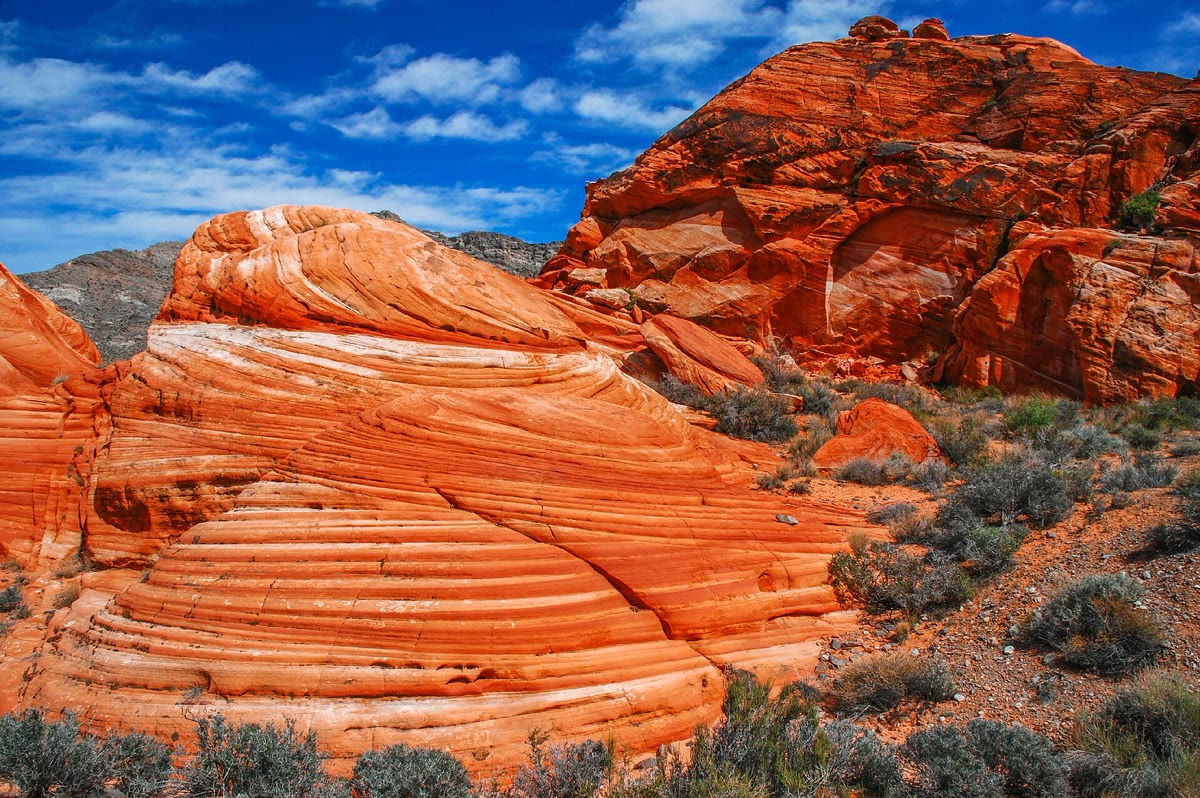
\includegraphics[height=3.6cm]{images/book3/b1-cross-bedding-aztec.jpg}};
\end{tikzpicture}

{\small Izquierda: la geometría de las \omterm{def:b1:clastic-sediments:bedform}{formas de fondo} ascendentes (esquemático, ángulos exagerados). Los valles recorren trayectorias rectas inclinadas según el ángulo de
ascenso $\theta$ (líneas gruesas); entre dos de ellas se conservan las partes inferiores de los foresets, en conjuntos de espesor $T = L\sin\theta$. Derecha: \omterm{def:b1:clastic-sediments:cross-bedding}{estratificación
cruzada} en la arenisca de Aztec, Muddy Mountains, Nevada: conjuntos inclinados de láminas, cada uno cortado en lo alto por la superficie de erosión de la base del siguiente.
Fotografía de Chip Carroon, Oficina de Gestión de Tierras, CC~BY-SA~2.0, a través de Wikimedia Commons.}
\label{fig:b1:clastic-sediments:climb}
\end{omfigure}
% ledger: southard:climb, commons:aztec-crossbed

\emph{\omterm{def:b1:clastic-sediments:cross-bedding}{Paleocorrientes}.} Las direcciones de \omterm{def:b1:geological-maps:attitude}{buzamiento} de las \omterm{def:b1:clastic-sediments:cross-bedding}{estratificaciones cruzadas} medidas en un afloramiento se dispersan alrededor de la dirección media de la corriente,
porque las caras de sotavento de \omterm{def:b1:clastic-sediments:bedform}{dunas} y \omterm{def:b1:clastic-sediments:bedform}{rizos} son curvas y las propias corrientes divagan. Su media se toma como media vectorial, no aritmética, por la razón mostrada en
\cref{prop:b1:field-lab-methods-1:vector-mean}: los \omterm{def:b1:spherical-astronomy:horizontal}{acimutes} son ángulos sobre un círculo, y 350 y 010 promedian 000, no 180.

\begin{proposition}[Media de acimutes]\label{prop:b1:clastic-sediments:azimuths}
Sean $\alpha_1, \ldots, \alpha_N$ \omterm{def:b1:spherical-astronomy:horizontal}{acimutes}, medidos en el sentido de las agujas del reloj desde el norte. Su media vectorial $\bar\alpha$ y su longitud media resultante $\bar R$ se
dan por
\[
  S = \sum_{i=1}^N \sin\alpha_i, \quad C = \sum_{i=1}^N \cos\alpha_i, \quad
  \bar\alpha = \operatorname{atan2}(S, C), \quad \bar R = \frac{\sqrt{S^2 + C^2}}{N},
\]
donde $\operatorname{atan2}(S, C)$ es el ángulo cuyos seno y coseno son proporcionales a $S$ y $C$, tomado entre \ang{0} y \ang{360}. $\bar R$ está entre 0 y 1, y vale 1 solo si
todos los \omterm{def:b1:spherical-astronomy:horizontal}{acimutes} son iguales.
\end{proposition}

\begin{proof}
El vector unitario del \omterm{def:b1:spherical-astronomy:horizontal}{acimut} $\alpha$, con el este como primera coordenada y el norte como segunda, es $(\sin\alpha, \cos\alpha)$. La suma de los $N$ vectores unitarios es
$(S, C)$, y su dirección, la media vectorial (\cref{def:b1:field-lab-methods-1:mean-orientation}), tiene el \omterm{def:b1:spherical-astronomy:horizontal}{acimut} cuyos seno y coseno son $S/\sqrt{S^2+C^2}$ y
$C/\sqrt{S^2+C^2}$. Por la desigualdad triangular, la longitud de una suma de $N$ vectores unitarios es a lo sumo $N$, con igualdad solo cuando todos apuntan
hacia el mismo lado.
\end{proof}

\begin{method}[Paleocorriente a partir de la estratificación cruzada]\label{met:b1:clastic-sediments:palaeocurrent}
\begin{enumerate}
  \item En cada conjunto, mídase la \omterm{def:b1:geological-maps:attitude}{dirección de buzamiento} de los foresets, eligiendo superficies que muestren su \omterm{def:b1:geological-maps:attitude}{buzamiento} verdadero (o mídase \omterm{def:b1:geological-maps:attitude}{rumbo} y \omterm{def:b1:geological-maps:attitude}{buzamiento}).
  \item Mídase la \omterm{def:b1:geological-maps:attitude}{actitud} de la estratificación principal; si está inclinada más de unos pocos grados, gírese cada foreset hasta la horizontal alrededor del \omterm{def:b1:geological-maps:attitude}{rumbo} de la
        estratificación (un giro hecho con la proyección estereográfica del volumen del año~3).
  \item Calcúlense la media vectorial $\bar\alpha$ y $\bar R$ de las direcciones de \omterm{def:b1:geological-maps:attitude}{buzamiento} corregidas (\cref{prop:b1:clastic-sediments:azimuths}).
  \item Represéntense las lecturas como un diagrama de rosa, un histograma circular de \omterm{def:b1:spherical-astronomy:horizontal}{acimutes}, para ver si forman un grupo o dos: las corrientes de marea que se invierten
        construyen conjuntos que buzan en sentidos opuestos, en la \omterm{def:b1:clastic-sediments:cross-bedding}{estratificación cruzada} en espina de pescado, y una media única carece entonces de sentido.
\end{enumerate}
\end{method}
% ledger: og:sorting-environments

\emph{Otras estructuras.} Varias otras estructuras registran las condiciones del depósito y el lado de arriba de los estratos. Un \omterm{def:b1:clastic-sediments:turbidite}{estrato gradado} se vuelve más fino hacia
arriba, de grueso en su base a fino en su techo, a medida que los granos se depositan de una corriente en descenso, los más gruesos primero (\cref{def:b1:clastic-sediments:turbidite}).
Las grietas de desecación, polígonos de grietas de retracción rellenas por la capa siguiente, se forman donde el lodo se seca al aire, como en las llanuras de marea y de inundación.
Las socavaciones que la corriente excava en el lodo de abajo, y que rellena la arena de arriba, se conservan como moldes en la base del estrato de arenisca, y sus formas indican
hacia dónde fue la corriente.
% ledger: og:sorting-environments

\section{Facies, ríos y deltas}\label{sec:b1:clastic-sediments:rivers-deltas}

La granulometría, la \omterm{def:b1:clastic-sediments:sorting}{clasificación}, las estructuras, los fósiles y la composición forman en conjunto el carácter de una roca sedimentaria, y los geólogos usan una sola palabra para ese carácter.

\begin{definition}[Facies sedimentaria, ambiente de depósito]\label{def:b1:clastic-sediments:facies}
Una \emph{facies sedimentaria}\index{facies sedimentaria} es un cuerpo de roca sedimentaria que se distingue de otros por su litología, tamaño de grano, estructuras sedimentarias
y fósiles, todos los cuales reflejan las condiciones en que se formó. El \emph{ambiente de depósito}\index{ambiente de depósito} es el lugar, con sus condiciones físicas, químicas
y biológicas, en el que se deposita un sedimento: un cauce de río, una llanura de inundación, una playa, la pendiente de un delta, el fondo del mar profundo.
\end{definition}
% ledger: og:sorting-environments

Una facies es una descripción, un ambiente una interpretación, y varios ambientes pueden producir la misma facies: la arena con \omterm{def:b1:clastic-sediments:bedform}{rizos} se deposita en ríos, en llanuras de marea y en el
fondo del mar profundo. La interpretación descansa, por tanto, en las asociaciones de facies y en el orden en que se apilan, que siguen el movimiento de los ambientes en el espacio: las
leyes generales de esa superposición, y los modelos estándar de cada ambiente, son el tema del volumen del año~3. Este capítulo describe los principales ambientes clásticos y las sucesiones
verticales que los identifican.

\emph{Ríos trenzados y meandriformes.} Los ríos vienen en dos estilos principales. Un río trenzado fluye por muchos canales que se separan y se reúnen alrededor de barras de grava y
arena; los ríos trenzados transportan cargas gruesas cerca de sus fuentes, al pie de las montañas o delante de los glaciares, y sus depósitos son \omterm{def:b1:layered-earth:layers}{mantos} de grava y de arena gruesa con
\omterm{def:b1:clastic-sediments:cross-bedding}{estratificación cruzada}, con poco lodo. Un río meandriforme fluye por un único canal sinuoso. El agua más rápida corre por el exterior de cada curva, donde erosiona la orilla cóncava; en el
interior, donde el agua es más lenta, se deposita arena sobre la barra de meandro. El meandro migra así lateralmente, erosionando de un lado y construyendo del otro; la llanura de inundación más
allá de las orillas recibe solo el lodo de las crecidas.
% ledger: og:rivers

La sucesión de la barra de meandro sigue de las \omterm{def:b1:clastic-sediments:bedform}{formas de fondo}. Al pie de la barra, en el agua más profunda y rápida, la corriente deja los granos más gruesos y construye \omterm{def:b1:clastic-sediments:bedform}{dunas}; subiendo por la
barra de pendiente suave el agua se hace más somera y lenta, la arena más fina, y las \omterm{def:b1:clastic-sediments:bedform}{dunas} ceden su lugar a los \omterm{def:b1:clastic-sediments:bedform}{rizos} (\cref{sec:b1:clastic-sediments:bedforms}); en lo alto, la barra pasa a la
llanura de inundación. Al migrar el meandro, cada una de estas zonas se desplaza sobre la que está debajo, y un sondeo a través del depósito las encuentra apiladas: una sucesión que se vuelve
más fina hacia arriba, desde una superficie de erosión hasta el lodo, una por cada paso de un canal, cuyo espesor es aproximadamente la profundidad del canal que la hizo.

\emph{Deltas.} Donde un río entra en una masa de agua en reposo, su corriente se extiende y se frena, y su carga se deposita: la carga gruesa cerca de la desembocadura, la fina más lejos. Un delta
crece hacia delante, o prograda, mientras el río aporte más sedimento del que el oleaje y las mareas pueden llevarse. Lo que el oleaje y las mareas hacen con el aporte decide su forma.

\begin{definition}[Deltas dominados por el río, por el oleaje y por la marea]\label{def:b1:clastic-sediments:delta}
Un delta es \emph{dominado por el río}\index{delta dominado por el río} cuando el aporte del río abruma al oleaje y a las mareas, y sus canales distributarios, encajados por sus propios
diques, construyen en el mar largos dedos de arena; es \emph{dominado por el oleaje}\index{delta dominado por el oleaje} cuando el oleaje retrabaja la arena llevada a las desembocaduras
hasta formar playas y cordones litorales a lo largo de una costa suave y arqueada; es \emph{dominado por la marea}\index{delta dominado por la marea} cuando las corrientes de marea, que entran y
salen por las desembocaduras, dan forma a su arena en barras y crestas paralelas al flujo, separadas por canales en forma de embudo.
\end{definition}
% ledger: og:deltas

\begin{omfigure}
\begin{tikzpicture}[font=\footnotesize, >={Stealth[length=4pt]}]
% meander in plan view (schematic) and the fining-upward log of a point bar
\begin{scope}[yscale=0.8]
  \fill[green!8] (-0.2,-0.4) rectangle (7.2,4.4);
  \draw[omSea!80!black, line width=9pt] plot[smooth, tension=0.7] coordinates {(0,3.6) (1.4,3.7) (2.6,2.8) (2.3,1.4) (3.2,0.5) (4.6,0.8) (5.0,2.2) (5.6,3.4) (7.0,3.5)};
  \draw[omSea!45, line width=7pt] plot[smooth, tension=0.7] coordinates {(0,3.6) (1.4,3.7) (2.6,2.8) (2.3,1.4) (3.2,0.5) (4.6,0.8) (5.0,2.2) (5.6,3.4) (7.0,3.5)};
  % point bars (inside of bends) with scroll lines
  \foreach \r in {0.25,0.45,0.65} {\draw[brown!60!black, densely dotted] (3.45,1.15) ++(200:\r) arc[start angle=200, end angle=340, radius=\r];}
  \fill[brown!25, opacity=0.8] (3.45,1.25) ellipse[x radius=0.55, y radius=0.35];
  \node[align=center] at (3.45,1.95) {barra de meandro\\ (depósito)};
  \fill[brown!25, opacity=0.8] (1.75,2.75) ellipse[x radius=0.4, y radius=0.45];
  \node[align=center] at (1.3,1.95) {barra de meandro};
  \draw[red!60!black, thick] (2.9,0.2) .. controls (3.3,0.0) and (4.3,0.15) .. (4.85,0.6);
  \node[red!60!black, anchor=north] at (4.0,0.0) {orilla erosionada};
  \draw[->, black!70] (5.9,3.0) -- (6.7,3.15) node[right] {flujo};
  \node[anchor=north west, black!60] at (5.2,1.3) {llanura de inundación};
  \node[font=\footnotesize] at (3.5,-0.85) {(a) un meandro, en planta};
\end{scope}
\begin{scope}[xshift=9.2cm, yshift=-0.3cm, yscale=0.8]
  % log: x width = grain size; y = height
  \draw[lith shale] (0,3.6) rectangle (0.8,4.6);
  \draw[lith sandstone] (0,2.6) rectangle (1.2,3.6);
  \draw[lith sandstone] (0,0.6) rectangle (1.7,2.6);
  \draw[lith conglomerate] (0,0) rectangle (2.2,0.6);
  \draw[very thick, red!60!black] (0,0) -- (2.2,0);
  % cross-bed symbols
  \foreach \y in {0.9,1.5,2.1} {\draw[black!70] (0.3,\y) .. controls (0.6,\y+0.05) and (0.9,\y+0.25) .. (1.2,\y+0.4);}
  \foreach \x in {0.2,0.5,0.8} {\draw[black!70] (\x,3.0) -- ++(0.12,0.1) -- ++(0.12,-0.1);}
  \node[anchor=west, align=left] at (2.4,4.1) {lodo de la llanura,\\ raíces, grietas de desecación};
  \node[anchor=west, align=left] at (2.4,3.1) {arena fina, laminación\\ cruzada de rizos};
  \node[anchor=west, align=left] at (2.4,1.6) {arena media a gruesa,\\ estratificación cruzada\\ de dunas};
  \node[anchor=west, align=left] at (2.4,0.3) {lag de grava sobre una\\ superficie de erosión};
  \draw[->] (-0.35,0) -- (-0.35,4.6) node[above] {arriba};
  \draw[<->, black!60] (-0.7,0) -- node[above, rotate=90, font=\scriptsize] {profundidad del canal} (-0.7,3.6);
  \node[font=\footnotesize, align=center] at (1.8,-0.5) {(b) sucesión de\\barra de meandro};
\end{scope}
\end{tikzpicture}

{\small (a)~Un río meandriforme (esquemático): la corriente erosiona la orilla exterior de cada curva y deposita arena sobre la barra de meandro del interior; las líneas
curvadas de rodillo son las posiciones sucesivas de la barra. (b)~La sucesión que deja una barra de meandro en migración, con el ancho de cada capa proporcional a su
tamaño de grano (esquemático). Se vuelve más fina hacia arriba, y su espesor registra la profundidad del canal.}
\label{fig:b1:clastic-sediments:point-bar}
\end{omfigure}
% ledger: og:rivers, southard:phase-diagram

Los tres miembros extremos son los vértices de un triángulo en el que cualquier delta puede situarse según la fuerza relativa de los tres procesos. El delta en pata de pájaro
del Misisipi, con sus largos dedos hacia el golfo de México (\cref{ch:b1:erosion-transport}), es el delta clásico \omterm{def:b1:clastic-sediments:delta}{dominado por el río}; el Nilo, con su arco suave de playas, uno
\omterm{def:b1:clastic-sediments:delta}{dominado por el oleaje}; el delta del Ganges y del Brahmaputra, el mayor del mundo, uno \omterm{def:b1:clastic-sediments:delta}{dominado por la marea}.
% ledger: og:deltas

\begin{omfigure}
\begin{tikzpicture}[font=\footnotesize]
% delta classification triangle (schematic) and the Lena delta from Landsat
\begin{scope}[yscale=0.82]
  \coordinate (R) at (2.6,4.5); \coordinate (W) at (0,0); \coordinate (T) at (5.2,0);
  \fill[omDef!8] (R) -- (W) -- (T) -- cycle;
  \draw[thick] (R) -- (W) -- (T) -- cycle;
  \node[above, align=center] at (R) {\textbf{dominado por el río}\\ dedos alargados, diques};
  \node[below, align=center] at (W) {\textbf{dominado por el oleaje}\\ cordones litorales suaves};
  \node[below, align=center] at (T) {\textbf{dominado por la marea}\\ barras paralelas al flujo};
  \fill[omThm] (2.6,2.9) circle[radius=2pt] node[below=1pt] {Mississippi};
  \fill[omThm] (0.75,0.4) circle[radius=2pt] node[above right=0pt] {Nile};
  \fill[omThm] (4.4,0.4) circle[radius=2pt] node[above left=0pt, align=right] {Ganges--\\ Brahmaputra};
\end{scope}
\node[anchor=south west, inner sep=0] at (7.2,-0.9) {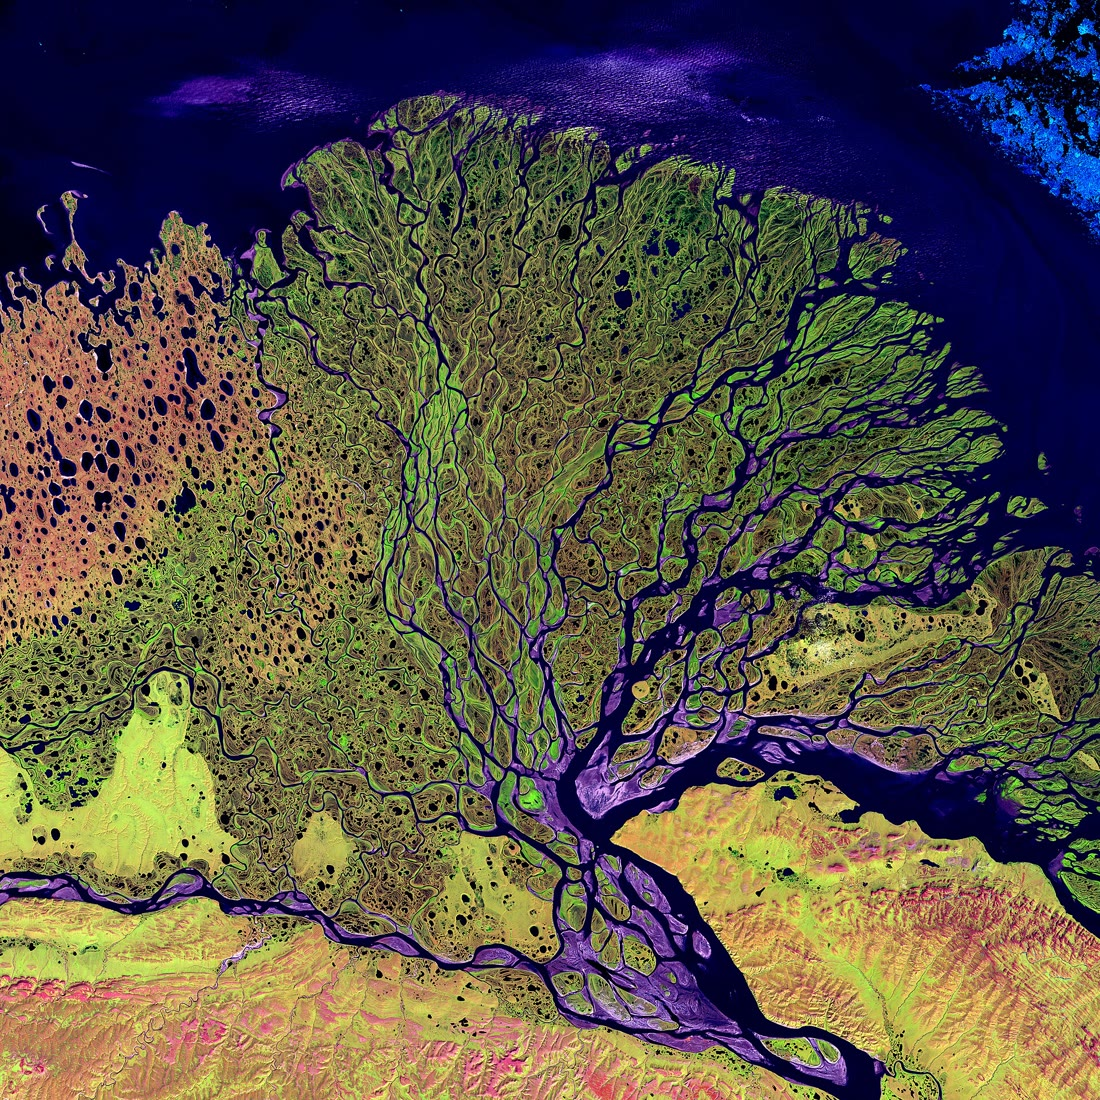
\includegraphics[height=5.2cm]{images/book3/b1-lena-delta.jpg}};
\end{tikzpicture}

{\small Izquierda: los tres miembros extremos de los deltas, según el proceso que los da forma (esquemático; las posiciones de los tres ejemplos son orientativas).
Derecha: el delta del Lena, en Siberia, que avanza sobre el mar de Laptev (arriba); el río entra por la derecha inferior y se divide en cientos de distributarios.
Imagen en falso color de Landsat~7 del 27 de febrero de 2000, Servicio Geológico de los Estados Unidos, dominio público, a través de Wikimedia Commons.}
\label{fig:b1:clastic-sediments:deltas}
\end{omfigure}
% ledger: og:deltas, commons:lena-delta

\emph{La sucesión que engrosa hacia arriba.} Delante de la desembocadura del río, el delta tiene un frente de pendiente suave, el frente deltaico, que pasa mar adentro al
prodelta, donde solo se asienta lodo desde la suspensión. Al progradar el delta, cada una de estas zonas avanza sobre la que tiene delante: un sondeo en la llanura deltaica encuentra,
de abajo arriba, los lodos laminados del prodelta, luego limo y arena alternados del frente deltaico inferior, luego la arena con \omterm{def:b1:clastic-sediments:cross-bedding}{estratificación cruzada} de las barras de desembocadura,
cortadas en lo alto por los canales de la llanura deltaica. La sucesión engrosa hacia arriba, lo contrario de una barra de meandro, y su espesor es aproximadamente la profundidad del agua
en la que progradó el delta. Su tasa está ligada a la geometría del frente deltaico.

\begin{proposition}[Progradación y acumulación]\label{prop:b1:clastic-sediments:progradation}
Sea un frente deltaico de pendiente constante $\alpha$ que avanza horizontalmente a la velocidad $v$ sin cambiar de forma, con nivel del mar constante. Un punto fijo bajo el frente
recibe entonces sedimento a la tasa vertical
\[
  a = v\,\tan\alpha,
\]
y la sucesión del frente deltaico de espesor $h$ se acumula allí en el tiempo $h/(v\tan\alpha)$.
\end{proposition}

\begin{proof}
En el tiempo $\mathrm dt$ el frente avanza $v\,\mathrm dt$. En un punto fijo bajo la superficie inclinada, la superficie sube la diferencia de altura entre dos puntos del frente separados
horizontalmente $v\,\mathrm dt$, es decir $v\,\mathrm dt\,\tan\alpha$, de donde la tasa. El frente cruza el punto mientras la superficie sube $h$, lo que tarda el tiempo $h/a$.
\end{proof}

Los frentes deltaicos tienen pendientes suaves, así que $\tan\alpha$ es pequeño: el frente de un delta avanza mucho más deprisa de lo que se acumula el sedimento en cualquier punto bajo él
(\cref{exo:b1:clastic-sediments:12}).

\begin{inthelab}[Describir un testigo]
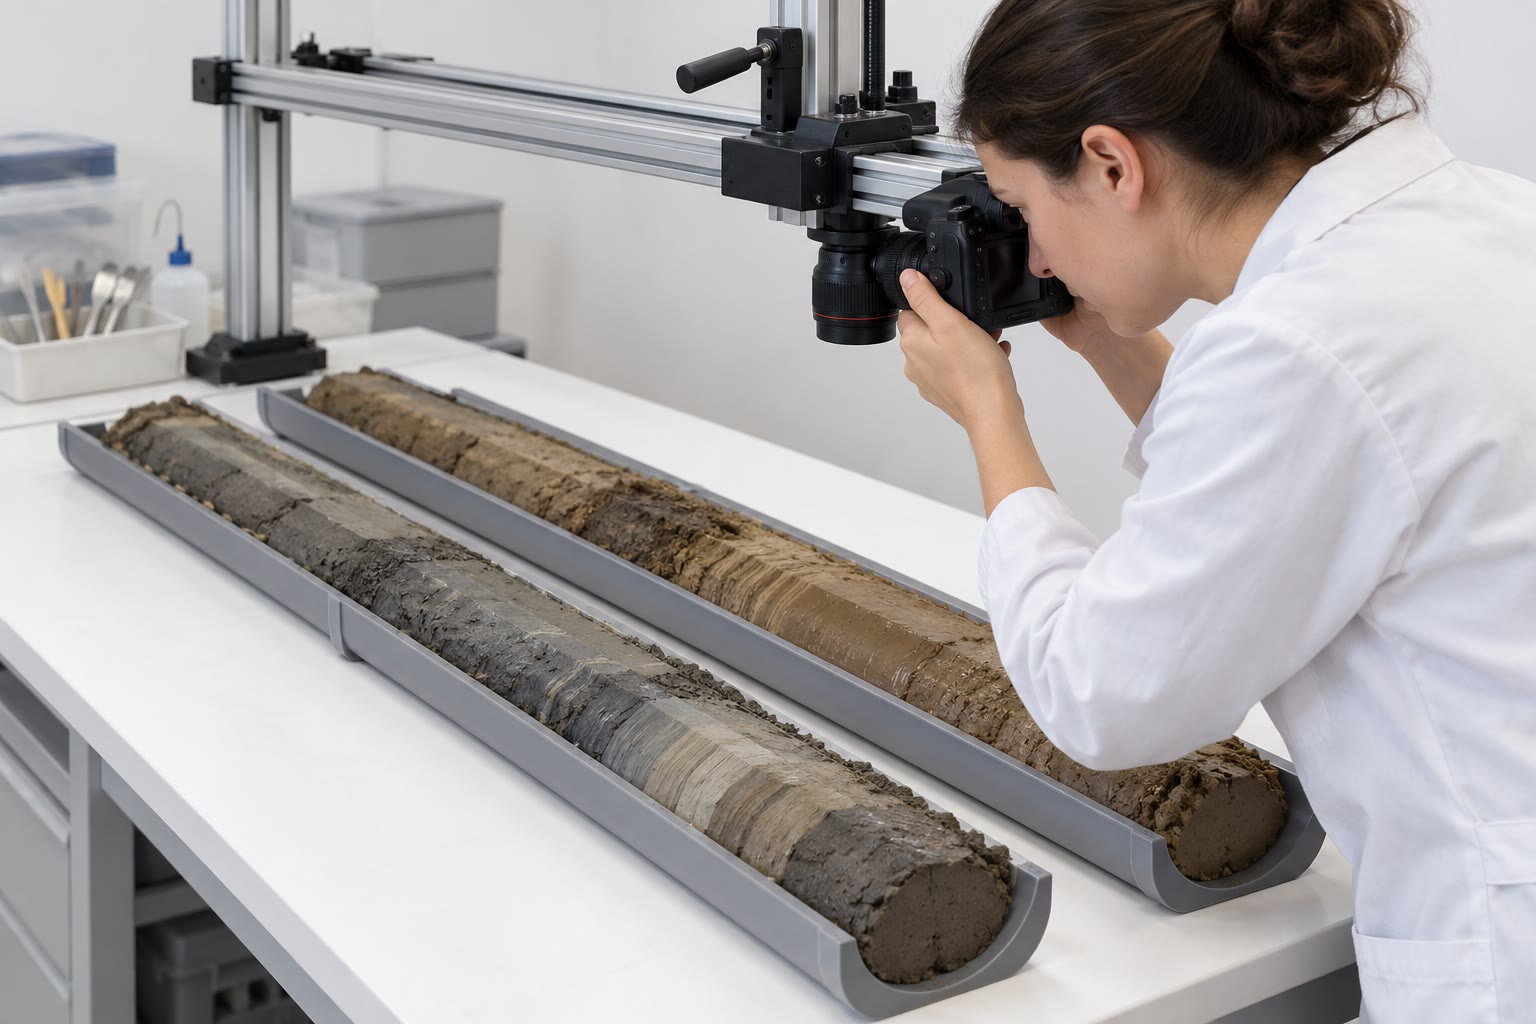
\includegraphics[width=0.3\linewidth]{images/book3/ai/b1-core-lab.jpg}\hfill
\begin{minipage}[b]{0.67\linewidth}
Los cilindros de sedimento o de roca que sube una perforadora se colocan en bandejas en orden de profundidad, se parten a lo largo y se fotografían con luz uniforme antes de que se
sequen y cambien de color. El sedimentólogo dibuja entonces un perfil del testigo, metro a metro: la litología, el tamaño de grano de cada capa (el ancho de la columna), las estructuras
(\omterm{def:b1:clastic-sediments:cross-bedding}{estratificación cruzada}, laminación, gradación, madrigueras), los \omterm{def:b1:geological-maps:geological-map}{contactos}, netos o graduales, el color y los fósiles. Se toman muestras para el análisis granulométrico y las \omterm{def:b1:field-lab-methods-1:thin-section}{láminas
delgadas}. Un testigo es una ventana estrecha: la dirección de la \omterm{def:b1:clastic-sediments:cross-bedding}{estratificación cruzada} se pierde a menos que el testigo esté orientado, y la extensión lateral de las capas debe venir de otras perforaciones.
\end{minipage}

\smallskip
{\small Un testigo dispuesto para fotografiarse en un laboratorio de sedimentos (ilustración IA).}
\end{inthelab}

\section{Costa y plataforma}\label{sec:b1:clastic-sediments:shoreline}

A lo largo de la costa entre los deltas, la arena que traen los ríos la moldean las olas y las mareas. Una playa es arena retrabajada por el swash, la delgada lámina de
agua que sube y baja por ella después de romper cada ola: los granos se mueven una y otra vez, los finos son llevados mar adentro, y las arenas de playa están entre las mejor clasificadas
y más redondeadas de todos los sedimentos. Sus láminas, depositadas por el swash, buzan suavemente hacia el mar. En muchas costas bajas la arena forma islas barrera, largos cordones de playa y
\omterm{def:b1:clastic-sediments:bedform}{dunas} eólicas separados del continente por lagunas, que son tranquilas y de grano fino, y conectadas con el mar por canales de marea.

Donde las mareas son fuertes y las olas débiles, la costa está bordeada por llanuras de marea, cubiertas y descubiertas dos veces al día. Pasan de arena cerca de la línea de bajamar, donde las
corrientes son más fuertes, a lodo cerca de la línea de pleamar, donde el agua en calma deja asentarse la arcilla; sus depósitos muestran el flujo invertido en la \omterm{def:b1:clastic-sediments:cross-bedding}{estratificación cruzada} en
espina de pescado, el secado en las grietas de desecación, y la alternancia de corriente y agua en calma en láminas finas de lodo que recubren arena con \omterm{def:b1:clastic-sediments:bedform}{rizos}.

Mar adentro, la plataforma es barrida por las olas solo hasta una profundidad que crece con el tamaño de las olas. Por encima de ella la arena se criba y se mueve; por debajo se asienta el lodo,
salvo durante las tormentas, cuando las olas mayores llegan más hondo y depositan \omterm{def:b1:layered-earth:layers}{mantos} de arena con la suave laminación ondulada llamada \omterm{def:b1:clastic-sediments:cross-bedding}{estratificación cruzada} en montículos (hummocky).
Una sucesión de plataforma alterna así a menudo el lodo de buen tiempo con las arenas de tormenta, más gruesas y espesas hacia la costa.
% ledger: og:sorting-environments, folk:maturity

\section{Clásticos de mar profundo}\label{sec:b1:clastic-sediments:deep-sea}

La arena y la grava también llegan a los fondos de los océanos profundos, a miles de metros de profundidad y a cientos de kilómetros de la tierra, y las transportan flujos que nadie ha visto
completos: corrientes densas, cargadas de sedimento, que bajan por el talud continental bajo el agua clara del océano.

\begin{history}[Cables en el fondo marino, 1929]
El 18 de noviembre de 1929 un terremoto de \omterm{def:b1:earthquake-source:mw}{magnitud de momento} 7.2 sacudió el talud continental al sur de Terranova, en el borde meridional de los Grandes Bancos. Un deslizamiento
de unos \qty{200}{km^3} de sedimento se movió por el talud, y un tsunami mató a 28 personas en la costa de Terranova. Doce cables telegráficos tendidos sobre el fondo del mar se
rompieron, algunos en varios puntos. Los más cercanos al epicentro se rompieron de inmediato; los demás, más al sur y más profundos, se rompieron uno tras otro en las horas siguientes,
por orden de distancia talud abajo. En 1952 Bruce Heezen y Maurice Ewing, al estudiar los momentos de las roturas, las explicaron: el deslizamiento se había convertido en una \omterm{def:b1:clastic-sediments:turbidite}{corriente
de turbidez} que bajó por el talud y se extendió por la llanura abisal más de 480 millas, rompiendo cada cable al pasar. A partir de los tiempos y las distancias estimaron su velocidad en
unos 50 nudos en el glacis continental superior, donde la pendiente es de alrededor del \qty{0.5}{\percent}, y aún 12 nudos en el último cable, a unas 400 millas de su origen. Al frenarse,
argumentaron, debió de depositar un \omterm{def:b1:clastic-sediments:turbidite}{estrato gradado} sobre la llanura, cada vez más fino hacia arriba.
\end{history}
% ledger: nrcan:grand-banks, he52:grand-banks

Cincuenta nudos son \qty{25.7}{m.s^{-1}}, más de \qty{90}{km.h^{-1}}, la velocidad de un coche en una carretera principal; 12 nudos son \qty{6.2}{m.s^{-1}}; y 480 millas son unos
\qty{770}{km}. Las roturas dieron también las primeras velocidades medidas de un flujo que se había inferido solo de sus depósitos y de experimentos en tanques.
% ledger: he52:grand-banks

\begin{definition}[Corriente de turbidez, turbidita, estrato gradado]\label{def:b1:clastic-sediments:turbidite}
Una \emph{corriente de turbidez}\index{corriente de turbidez} es una corriente de agua hecha más densa que el agua que la rodea por el sedimento que lleva en suspensión, que fluye talud
abajo bajo esa agua, con sus granos mantenidos en suspensión por la turbulencia que crea su propio movimiento. Una \emph{turbidita}\index{turbidita} es el depósito de una corriente de
turbidez. Un \emph{estrato gradado}\index{estrato gradado} es un estrato cuyo tamaño de grano disminuye desde su base hasta su techo.
\end{definition}
% ledger: og:sorting-environments, he52:grand-banks

Una \omterm{def:b1:clastic-sediments:turbidite}{corriente de turbidez} se impulsa a sí misma: corre porque su suspensión es pesada, y mantiene su suspensión porque corre. En una pendiente empinada puede recoger más sedimento del
fondo, hacerse más densa y acelerar; en la pendiente suave de la llanura abisal se frena, deja caer su carga y muere.

\begin{proposition}[Velocidad de una corriente de turbidez]\label{prop:b1:clastic-sediments:turbidity}
Una \omterm{def:b1:clastic-sediments:turbidite}{corriente de turbidez} de espesor $h$ y densidad $\rho + \Delta\rho$ fluye de manera estacionaria talud abajo, con pendiente $S$, bajo agua de densidad $\rho$. Si la resistencia
del fondo y del agua de encima es $\tau = \rho\,C_f\,U^2$ por unidad de área, siendo $C_f$ un coeficiente de fricción adimensional, su velocidad media es
\[
  U = \sqrt{\frac{\Delta\rho}{\rho}\,\frac{g\,h\,S}{C_f}} .
\]
\end{proposition}

\begin{proof}
El argumento es el del producto profundidad--pendiente (\cref{prop:b1:erosion-transport:depth-slope}), con el peso sustituido por el exceso de peso.
Una columna de la corriente de área unitaria pesa $(\rho +
\Delta\rho) g h$, y el agua que desaloja $\rho g h$:
en el agua circundante, solo el exceso $\Delta\rho\,g\,h$ la arrastra talud abajo, con la componente
$\Delta\rho\,g\,h\,S$ a lo largo de él. En flujo estacionario esto equilibra la resistencia $\rho C_f U^2$, de donde $U^2 = (\Delta\rho/\rho)\,g\,h\,S/C_f$.
\end{proof}

La ley de resistencia $\tau = \rho C_f U^2$, cuadrática en la velocidad, es la de los flujos turbulentos de la hidráulica (los libros de física), y $C_f$ se halla por experimento. La fórmula
desprecia el agua que la corriente mezcla consigo misma por su superficie superior, lo que la diluye y la frena. Muestra el papel de los tres factores: una corriente el doble de espesa, o el doble de
densa, o sobre una pendiente el doble de empinada, corre $\sqrt 2$ veces más deprisa. Una suspensión que lleva la fracción $c$ de su volumen como granos de cuarzo tiene
$\Delta\rho/\rho = 1.65\,c$ (\cref{sec:b1:erosion-transport:settling}), pequeño a menos que el flujo esté muy concentrado; ahí es donde una \omterm{def:b1:clastic-sediments:turbidite}{corriente de turbidez} difiere de un río, en el que
todo el peso del agua, no un pequeño exceso, impulsa el flujo. Para correr a los 50 nudos de 1929 en una pendiente de medio por ciento, una \omterm{def:b1:clastic-sediments:turbidite}{corriente de turbidez} necesita un producto grande
de espesor y exceso de densidad (\cref{exo:b1:clastic-sediments:11}).

\emph{La secuencia de Bouma.} En 1962 Arnold Bouma describió el orden interno de los estratos de arenisca de las sucesiones antiguas de mar profundo en cinco divisiones, rotuladas de abajo
arriba. A: arena masiva o gradada, a menudo sobre una base erosiva; B: arena con laminación paralela; C: arena fina con laminación cruzada de \omterm{def:b1:clastic-sediments:bedform}{rizos}, a menudo convoluta; D: limo laminado que
pasa a lodo; E: lodo. El orden se lee como el registro de una sola corriente en descenso que pasa sobre un punto: a medida que se frena, deja caer primero sus granos más gruesos en masa,
luego construye un lecho plano superior, luego \omterm{def:b1:clastic-sediments:bedform}{rizos}, y luego deja asentarse el limo y la arcilla. Las secuencias completas son raras: las divisiones superiores las erosiona a menudo la
corriente siguiente, y lejos del origen, donde la corriente es débil, faltan las inferiores.
% ledger: og:sorting-environments, shanmugam:bouma

\begin{omfigure}
\begin{tikzpicture}[font=\footnotesize]
% Bouma sequence: log (schematic) and a labelled photograph
\begin{scope}
  \draw[lith shale] (0,4.0) rectangle (0.7,4.8);
  \draw[lith shale] (0,3.3) rectangle (0.9,4.0);
  \draw[lith sandstone] (0,2.2) rectangle (1.3,3.3);
  \draw[lith sandstone] (0,1.2) rectangle (1.6,2.2);
  \draw[lith sandstone] (0,0) rectangle (2.0,1.2);
  \draw[very thick, red!60!black] (0,0) .. controls (0.6,-0.12) and (1.4,0.1) .. (2.0,0);
  \foreach \y in {1.4,1.6,1.8,2.0} {\draw[black!70] (0.1,\y) -- (1.5,\y);}
  \foreach \x in {0.15,0.5,0.85} {\draw[black!70] (\x,2.55) .. controls (\x+0.12,2.75) .. (\x+0.3,2.6);}
  \foreach \y in {3.45,3.6,3.75,3.9} {\draw[black!60] (0.1,\y) -- (0.8,\y);}
  \foreach \x/\y in {0.4/0.3, 0.9/0.5, 1.4/0.25, 0.6/0.8, 1.2/0.9} {\fill[black!60] (\x,\y) circle[radius=0.06];}
  \node[anchor=west] at (2.2,4.4) {E \quad lodo};
  \node[anchor=west] at (2.2,3.65) {D \quad limo laminado a lodo};
  \node[anchor=west] at (2.2,2.75) {C \quad laminación cruzada de rizos};
  \node[anchor=west] at (2.2,1.7) {B \quad laminación paralela};
  \node[anchor=west] at (2.2,0.6) {A \quad arena gradada};
  \node[anchor=west, red!60!black] at (2.2,-0.15) {base erosiva, marcas de base};
  \draw[->] (-0.3,0) -- (-0.3,4.8) node[above] {arriba};
\end{scope}
\node[anchor=south west, inner sep=0] at (6.9,-0.3) {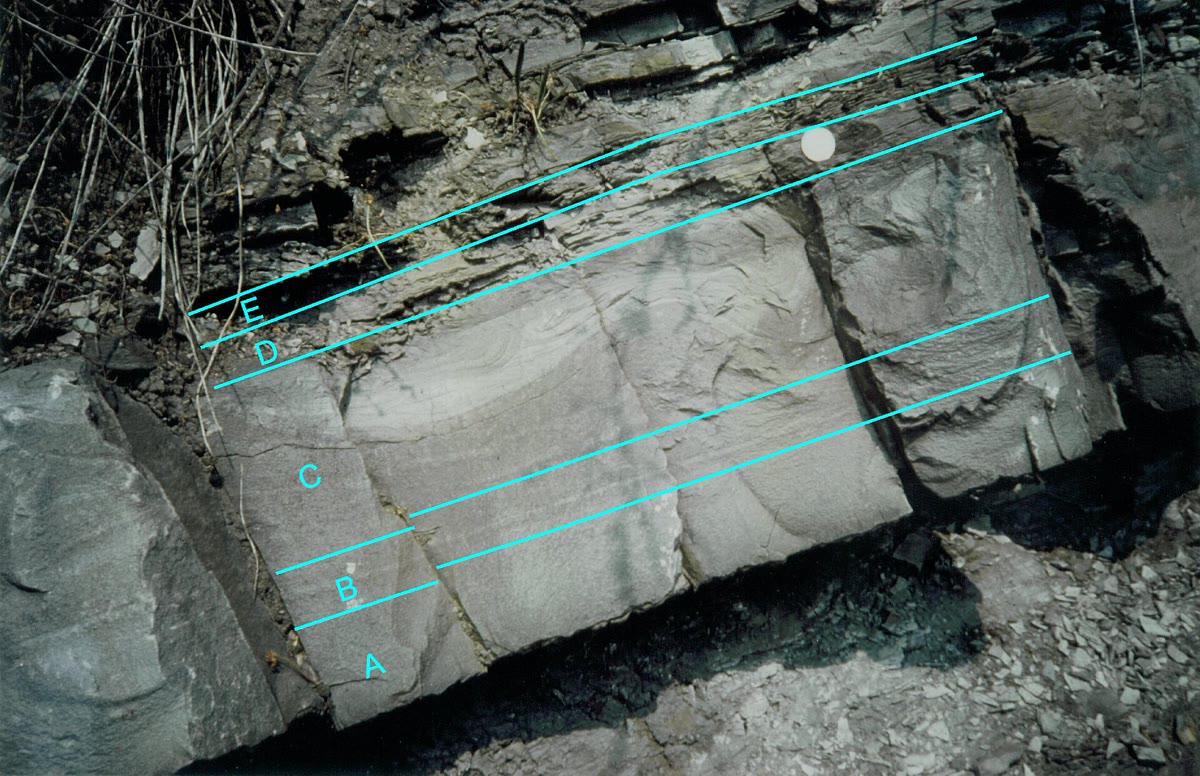
\includegraphics[height=5.2cm]{images/book3/b1-turbidite-bouma.jpg}};
\end{tikzpicture}

{\small Izquierda: las cinco divisiones de la secuencia de Bouma, con el ancho de cada una proporcional a su tamaño de grano (esquemático). Derecha: un estrato de \omterm{def:b1:clastic-sediments:turbidite}{turbidita} del
Devónico superior de Becke-Oese, Alemania, con las divisiones de la A a la E señaladas por el fotógrafo; la moneda da la escala. Fotografía de Jo Weber, CC~BY-SA~3.0, a través de
Wikimedia Commons.}
\label{fig:b1:clastic-sediments:bouma}
\end{omfigure}
% ledger: og:sorting-environments, shanmugam:bouma, commons:bouma-becke-oese

La secuencia de Bouma se convirtió en el modelo estándar de la \omterm{def:b1:clastic-sediments:turbidite}{turbidita}, y miles de areniscas antiguas de mar profundo se interpretaron con ella. La interpretación está
en disputa: las corrientes que corren a lo largo del talud, las corrientes profundas de marea y las ondas internas también construyen arenas con \omterm{def:b1:clastic-sediments:bedform}{rizos} y laminadas, y algunos
sedimentólogos sostienen que muchos estratos leídos como \omterm{def:b1:clastic-sediments:turbidite}{turbiditas}, incluidos algunos del área tipo, se depositaron por otros flujos. Se han observado pocas \omterm{def:b1:clastic-sediments:turbidite}{corrientes de turbidez}
en el océano actual, mientras que las \omterm{def:b1:clastic-sediments:turbidite}{turbiditas} antiguas se cuentan por miles.
% ledger: shanmugam:bouma

No todos los clásticos de mar profundo son \omterm{def:b1:clastic-sediments:turbidite}{turbiditas}. Las corrientes de contorno, las corrientes lentas y profundas que siguen las curvas de nivel del talud continental, retrabajan
el sedimento del talud en derivas alargadas y suaves, los contorníticos. Y lejos de los continentes, donde no llegan ni las \omterm{def:b1:clastic-sediments:turbidite}{corrientes de turbidez} ni las de contorno, el fondo del mar
recibe solo lo que se asienta desde el agua de encima: las conchas del plancton y el polvo eólico más fino, los sedimentos pelágicos del capítulo siguiente
(\cref{ch:b1:chemical-biogenic-sediments}).
% ledger: og:sorting-environments

\section{Ejercicios}

\begin{exercise}[$\star$]\label{exo:b1:clastic-sediments:1}
Conviértanse a unidades phi los diámetros \qty{0.18}{mm}, \qty{0.75}{mm}, \qty{3}{mm}, \qty{0.012}{mm} y \qty{150}{mm}, con dos decimales, y nómbrese la clase de cada uno
(\cref{tab:b1:clastic-sediments:classes}).
% ledger: folk:wentworth-classes
\end{exercise}

\begin{exercise}[$\star$]\label{exo:b1:clastic-sediments:2}
La curva acumulada de una arena de río da $\varphi_5 = 0.62$, $\varphi_{16} =
1.05$, $\varphi_{50} = 1.71$, $\varphi_{84} = 2.43$ y $\varphi_{95} = 2.98$.
Calcúlese su media gráfica, en unidades phi y en milímetros, y su desviación típica gráfica inclusiva, y nómbrese su tamaño y su \omterm{def:b1:clastic-sediments:sorting}{clasificación}.
% ledger: folk:graphic-measures, folk:sorting-classes
\end{exercise}

\begin{exercise}[$\star$]\label{exo:b1:clastic-sediments:3}
Unos \omterm{def:b1:clastic-sediments:bedform}{rizos} de \qty{2}{cm} de altura migran a \qty{1}{cm} por minuto sobre un fondo de arena de cuarzo de porosidad \num{0.4}. Con \cref{prop:b1:clastic-sediments:migration},
calcúlese el volumen de \omterm{def:b1:erosion-transport:load}{carga de fondo} por unidad de anchura, en \si{m^2.s^{-1}}, y la masa de cuarzo ($\qty{2650}{kg.m^{-3}}$) transportada sobre un metro de cresta en un día.
% ledger: hom:quartz
\end{exercise}

\begin{exercise}[$\star$]\label{exo:b1:clastic-sediments:4}
Un nudo es una milla náutica, \qty{1852}{m}, por hora. (a)~Conviértanse a metros por segundo las velocidades de 50 y 12 nudos estimadas para la \omterm{def:b1:clastic-sediments:turbidite}{corriente de turbidez} de
1929. (b)~¿Cuánto tarda una corriente a 12 nudos en recorrer \qty{100}{km}? (c)~Conviértanse 480 y 400 millas a kilómetros (una milla son \qty{1.609}{km}).
% ledger: he52:grand-banks
\end{exercise}

\begin{exercise}[$\star\star$]\label{exo:b1:clastic-sediments:5}
(a)~Usando los percentiles de una distribución normal dados en la demostración de \cref{prop:b1:clastic-sediments:normal}, calcúlese la desviación típica gráfica
$(\varphi_{84} - \varphi_{16})/2$ y la estimación $(\varphi_{95} - \varphi_5)/3.3$ para una distribución normal de desviación típica $\sigma$. (b)~¿Por qué podrían discrepar
las dos para un sedimento real? ¿Qué clase de sedimento las hace diferir más?
\end{exercise}

\begin{exercise}[$\star\star$]\label{exo:b1:clastic-sediments:6}
Un depósito de \omterm{def:b1:clastic-sediments:bedform}{rizos} ascendentes muestra conjuntos de \qty{1.5}{cm} de espesor, medidos perpendicularmente a sus límites, formados por \omterm{def:b1:clastic-sediments:bedform}{rizos} espaciados \qty{15}{cm}. (a)~Calcúlese el
ángulo de ascenso. (b)~Si los \omterm{def:b1:clastic-sediments:bedform}{rizos} se movieran a \qty{0.5}{cm} por minuto, ¿a qué velocidad se elevó el fondo, en centímetros por hora? (c)~¿Qué dice una velocidad así sobre el flujo?
% ledger: southard:climb
\end{exercise}

\begin{exercise}[$\star\star$]\label{exo:b1:clastic-sediments:7}
Seis direcciones de \omterm{def:b1:geological-maps:attitude}{buzamiento} de \omterm{def:b1:clastic-sediments:cross-bedding}{estratificación cruzada}, ya corregidas por la inclinación de los estratos, dan 350, 020, 005, 340, 015 y 030. (a)~Calcúlese su media aritmética.
(b)~Calcúlense su media vectorial y $\bar R$. (c)~Explíquese la diferencia.
\end{exercise}

\begin{exercise}[$\star\star$]\label{exo:b1:clastic-sediments:8}
Tres areniscas se examinan en \omterm{def:b1:field-lab-methods-1:thin-section}{lámina delgada}. A tiene un \qty{12}{\percent} de matriz arcillosa y granos angulosos de cuarzo, \omterm{def:b1:rock-forming-minerals:groups}{feldespato} y fragmentos de roca. B tiene un
\qty{2}{\percent} de arcilla, $\sigma_I = 0.40\,\varphi$ y granos de cuarzo de redondez \num{2.2} en la escala de Folk. C no tiene arcilla, $\sigma_I =
0.30\,\varphi$, granos de cuarzo de redondez \num{3.6}, y un \qty{98}{\percent} de cuarzo. Nómbrese la \omterm{def:b1:clastic-sediments:maturity}{madurez textural} de cada una, y sugiérase un \omterm{def:b1:clastic-sediments:facies}{ambiente de depósito} para cada una.
% ledger: folk:maturity
\end{exercise}

\begin{exercise}[$\star\star$]\label{exo:b1:clastic-sediments:9}
(a)~Calcúlese el número de Froude de un flujo de \qty{0.3}{m} de profundidad a \qty{1.5}{m.s^{-1}}, y el de un río de \qty{2}{m} de profundidad a \qty{1.0}{m.s^{-1}}
($g
= \qty{9.81}{m.s^{-2}}$). (b)~¿A qué profundidad un flujo de \qty{1.5}{m.s^{-1}} alcanzaría un número de Froude de 1, y qué velocidad necesitaría el río de \qty{2}{m} de profundidad?
(c)~¿Por qué son comunes las antidunas en las láminas de agua que bajan de una playa, y raras en los grandes ríos?
% ledger: southard:ripples-dunes
\end{exercise}

\begin{exercise}[$\star\star\star$]\label{exo:b1:clastic-sediments:10}
Un análisis por tamizado de una arena da, en clases phi enteras desde $-1$ hasta $5\,\varphi$: 2, 8, 30, 40, 15 y 5 por ciento en peso. (a)~Por el método de los momentos,
calcúlense la media y la desviación típica en unidades phi, y nómbrese la \omterm{def:b1:clastic-sediments:sorting}{clasificación}. (b)~Constrúyase la curva acumulada, léanse $\varphi_5$, $\varphi_{16}$, $\varphi_{50}$, $\varphi_{84}$ y
$\varphi_{95}$ por interpolación lineal, y calcúlense $M_z$ y $\sigma_I$. (c)~Compárense.
% ledger: folk:graphic-measures, folk:sorting-classes
\end{exercise}

\begin{exercise}[$\star\star\star$]\label{exo:b1:clastic-sediments:11}
Tómese $C_f = 0.003$ en \cref{prop:b1:clastic-sediments:turbidity}. (a)~Una \omterm{def:b1:clastic-sediments:turbidite}{corriente de turbidez} de \qty{50}{m} de espesor, con un exceso de densidad de
\qty{2}{\percent}, baja por una pendiente de \num{0.005}: calcúlese su velocidad, en metros por segundo y en nudos. (b)~¿Qué producto de espesor y exceso relativo de densidad
daría los 50 nudos de 1929 en la misma pendiente? (c)~La misma corriente que en (a) llega a una pendiente de \num{0.001}: calcúlese su nueva velocidad, si nada más cambia.
¿Qué le pasa a su carga?
% ledger: he52:grand-banks
\end{exercise}

\begin{exercise}[$\star\star\star$]\label{exo:b1:clastic-sediments:12}
Un río entrega \qty{50}{Mt} de sedimento al año a su delta, de los que el \qty{70}{\percent} se deposita en un frente deltaico de \qty{100}{km} de anchura que avanza en agua de
\qty{30}{m} de profundidad. El depósito tiene una densidad aparente de \qty{2000}{kg.m^{-3}}. (a)~¿Qué volumen añade cada año? (b)~Si este volumen llena toda la profundidad de agua a lo
largo de la anchura del frente, ¿con qué rapidez avanza el frente? (c)~Con una pendiente del frente deltaico de \ang{0.5}, ¿a qué tasa se acumula el sedimento en un punto fijo bajo el frente, y en
cuántos años se forma allí la sucesión que engrosa hacia arriba?
\end{exercise}

\section{Problema: lectura de un testigo de un delta}

\begin{problem}[{Problema de fin de semana --- un sondeo a través de un delta antiguo, desde los tamaños de grano hasta la dirección de sus ríos}]
\label{pb:b1:clastic-sediments:1}
% values: calc/ch21.py; the borehole, its beds, ages and readings are invented
Un sondeo atraviesa \qty{24}{m} de areniscas y lutitas depositadas por un delta antiguo. El geólogo describe cuatro unidades, de abajo arriba, y analiza una muestra de cada una.

\smallskip
\begin{center}\small
\begin{tabular}{@{}llccccc@{}}
\hline
unidad (profundidad) & descripción & $\varphi_5$ & $\varphi_{16}$ & $\varphi_{50}$ & $\varphi_{84}$ & $\varphi_{95}$ \\
\hline
1 (0--8 m) & lodolita gris laminada & 4.2 & 5.0 & 6.6 & 8.4 & 9.6 \\
2 (8--16 m) & limolita y arenisca alternadas & 1.9 & 2.4 & 3.4 & 4.6 & 5.5 \\
3 (16--21 m) & arenisca con \omterm{def:b1:clastic-sediments:cross-bedding}{estratificación cruzada} & 0.9 & 1.25 & 1.8 & 2.35 & 2.7 \\
4 (21--24 m) & arenisca con cantos, base erosiva & $-1.8$ & $-0.8$ & 0.9 & 2.1 & 2.9 \\
\hline
\end{tabular}
\end{center}

\medskip
\noindent\textbf{Parte I --- Los tamaños de grano.}
\begin{enumerate}
  \item Calcúlese la media gráfica $M_z$ de cada unidad, en unidades phi y en milímetros.
  \item Calcúlese la desviación típica gráfica inclusiva $\sigma_I$ de cada unidad.
  \item Nómbrese la clase de tamaño de la media y la \omterm{def:b1:clastic-sediments:sorting}{clasificación} de cada unidad.
  \item ¿Qué unidad está mejor clasificada? ¿Por qué una barra de desembocadura estaría mejor clasificada que los lodos del prodelta?
  \item Interpolando linealmente entre $\varphi_{50}$ y $\varphi_{84}$, estímese el porcentaje de partículas del tamaño de la arcilla (más finas que $8\,\varphi$) en la unidad~1.
        ¿Qué dice sobre las corrientes donde se depositó?
  \item ¿Por qué la curva acumulada de la unidad~4 está tan extendida, aunque es una arena de canal?
\end{enumerate}

\medskip
\noindent\textbf{Parte II --- La sucesión.}
\begin{enumerate}[resume]
  \item Descríbase cómo cambia el tamaño medio de la unidad~1 a la~3. ¿La sucesión se vuelve más fina o más gruesa hacia arriba?
  \item Interprétense las unidades 1, 2 y 3 como partes de un delta. ¿Qué zona del delta estaba en el lugar cuando se depositó cada una?
  \item ¿Qué muestra la superposición de las tres unidades sobre el movimiento del delta?
  \item ¿Qué profundidad de agua, como mínimo, alcanzó a construir el delta, y por qué?
  \item La unidad~4 tiene una base erosiva y es más gruesa que la~3. Interprétese.
  \item ¿Daría una barra de meandro la misma sucesión? Explíquese.
\end{enumerate}

\medskip
\noindent\textbf{Parte III --- ¿Con qué rapidez avanzó el delta?}
Dos finas capas de ceniza volcánica, en la base de la unidad~1 y en el techo de la unidad~2, están datadas; distan \num{4000}~años entre sí.
\begin{enumerate}[resume]
  \item Calcúlese la tasa media de acumulación entre las dos cenizas, en milímetros al año.
  \item El frente deltaico tenía una pendiente de \ang{0.5}. Con
        \cref{prop:b1:clastic-sediments:progradation}, calcúlese la velocidad a la que avanzó, en metros al año.
  \item ¿Cuánto avanzó el frente durante los \num{4000}~años?
  \item ¿Cuánto tardaron en acumularse en el lugar los 21 metros de las unidades 1 a 3, a esta tasa?
  \item ¿Por qué la tasa de acumulación de un delta no es la misma en todas partes al mismo tiempo?
\end{enumerate}

\medskip
\noindent\textbf{Parte IV --- ¿Por dónde fluían los ríos?}
Sobre la arenisca con \omterm{def:b1:clastic-sediments:cross-bedding}{estratificación cruzada} de la unidad~3, expuesta en un afloramiento cercano donde los estratos son horizontales, se miden doce direcciones de \omterm{def:b1:geological-maps:attitude}{buzamiento}
de foresets: 352, 010, 025, 004, 338, 017, 031, 359, 012, 046, 006 y 344.
\begin{enumerate}[resume]
  \item Calcúlese la media aritmética de las doce lecturas. ¿Tiene sentido?
  \item Calcúlense las sumas $S$ y $C$ de \cref{prop:b1:clastic-sediments:azimuths}.
  \item Calcúlese la longitud media resultante $\bar R$. ¿Son consistentes las lecturas?
  \item ¿En qué dirección general construyó el delta, y dónde estaba la tierra?
  \item ¿Por qué deben girarse las direcciones de \omterm{def:b1:geological-maps:attitude}{buzamiento} si los estratos están inclinados, y en torno a qué eje?
  \item ¿Pudo una corriente de marea construir estas \omterm{def:b1:clastic-sediments:cross-bedding}{estratificaciones cruzadas}? ¿Cómo sería su diagrama de rosa?
  \item Al grado más próximo, ¿cuál es el \omterm{def:b1:spherical-astronomy:horizontal}{acimut} medio de la \omterm{def:b1:clastic-sediments:cross-bedding}{paleocorriente} de la arenisca con \omterm{def:b1:clastic-sediments:cross-bedding}{estratificación cruzada} de la unidad~3?
\end{enumerate}
\end{problem}
